\documentclass[11pt, oneside]{article}   	% use "amsart" instead of "article" for AMSLaTeX format
\usepackage{geometry}                		% See geometry.pdf to learn the layout options. There are lots.
\geometry{a4paper}                   		% ... or a4paper or a5paper or ... 
%\geometry{landscape}                		% Activate for for rotated page geometry
%\usepackage[parfill]{parskip}    		% Activate to begin paragraphs with an empty line rather than an indent
\usepackage{graphicx}				% Use pdf, png, jpg, or eps§ with pdflatex; use eps in DVI mode
\usepackage{array}							% TeX will automatically convert eps --> pdf in pdflatex		
\usepackage{amssymb}
\usepackage{hyperref}
\usepackage{cite}
\usepackage[final]{fixme}
\usepackage{pdfpages}
\usepackage{tabularx}
\usepackage{fancyheadings}
\usepackage{lastpage}
\usepackage{float}
\restylefloat{table}


\parskip 6pt % 1pt = 0.351 mm
\parindent 0pt

%\title{Requirement Engineering Process in AMIDST}
%\author{The handsome AMIDST guys et. al.}
%\date{Latest version, \today}							% Activate to display a given date or no date

\pagestyle{fancy}
\lhead{\tiny FP7-ICT 619209 / AMIDST}
\chead{\tiny Page {\thepage} of \pageref{LastPage} \\}
\rhead{\tiny Public}
\renewcommand{\footrulewidth}{0.4pt}
\cfoot{}



\begin{document}

%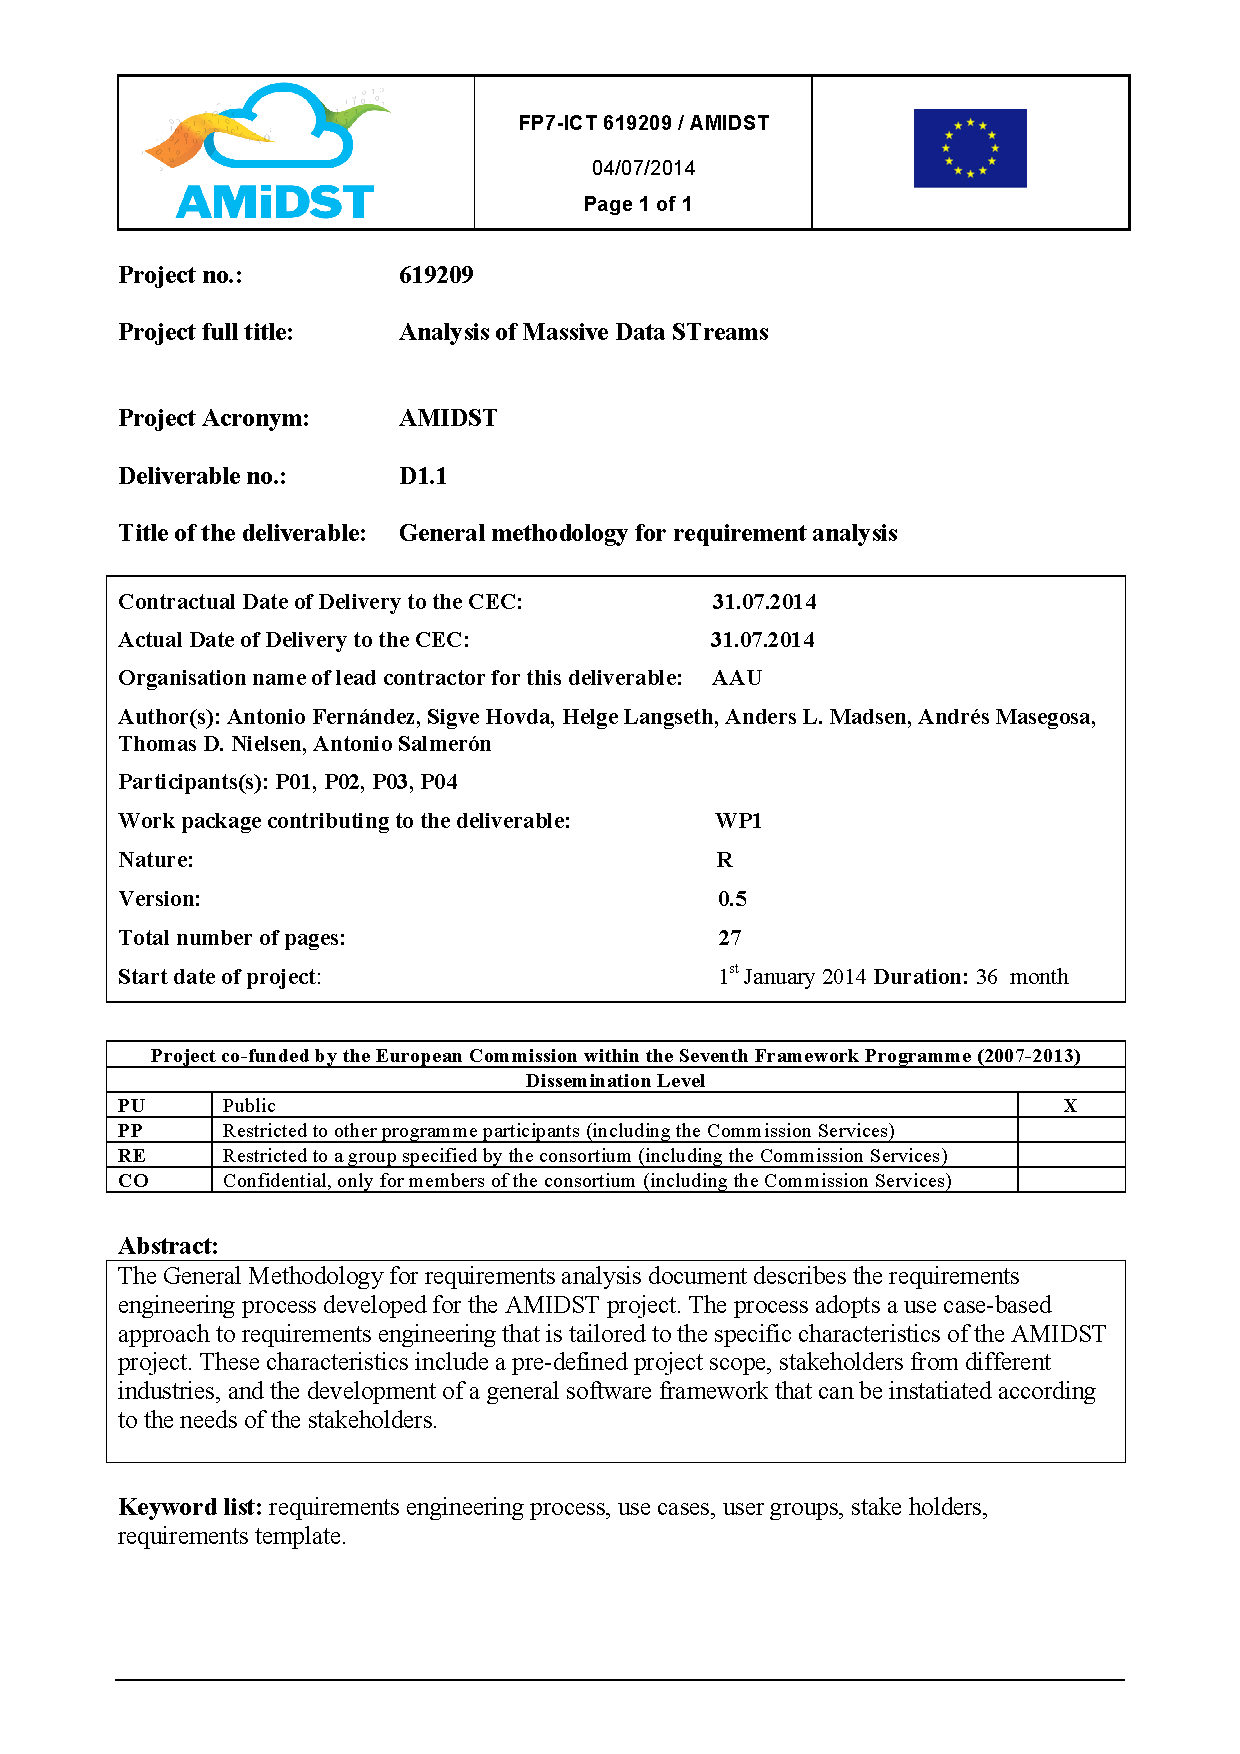
\includepdf{AMiDST_Template_Deliverables.pdf}

%\maketitle
%
%\begin{abstract}
%\end{abstract}
%



% Table of contents
\tableofcontents

\newpage

% Document History

\section*{Document history}

\begin{table}[htbp]
  \centering
  \begin{tabularx}{\linewidth}{|p{17mm}|p{17mm}|X|X|}\hline
    {\bf Version} & {\bf Date} & {\bf Author (Unit)} & {\bf Description} \\ \hline \hline
    v0.3 &  &  & First draft finished  \\ 
\hline
  \end{tabularx}
\end{table}

\newpage


% Document History

\section{Executive summary}

The aim of this document is to track the development of the coding of the AMIDST toolbox. The document is structured by the different use cases of the toolbox.  For each use case (included in independent sections),  we include a description of the purpose of the use case as well as a categorized list of the associated requirements. We then associate to each use case a list of so-called \textit{\textbf{functionalities}} (included in independent subsections) that are coded in the toolbox to cover the specific use case and their associated requirements. A \textit{functionality}, or also called a \textit{feature}, is a set of java classes which allow to perform a specific task or which define a coherent concept within the toolbox. For example, the creation and managing of random variables, reading a data set from a file, building and handling dynamic Bayesian networks, the maximum likelihood estimation etc. The set of \textit{functionalities} identify those key parts of the toolbox that any developer or toolbox user need to understand in order to make a proper use of the software tool

Another important part of this document is to detail the time line of the toolbox development. Each of the use cases contain a subsection titled \textit{Time Tables} which contain details about the development phase of each one of the \textit{functionalities} associated to this use case. Six main phases are identified: design, prototype, code-review, testing, documentation and (first) release. Looking at this section we can easily track the evolution of the use case.

In the last section we detail the class diagram of each code package of the toolbox. The document is concluded with an appendix which contains a pdf document generated by the toolbox Doxygen and which contain all the java docs of all the coded java classes. 


We highlight that the contents detailed here can be later transformed or reorganized to create the different deliverables and the final user-manual of this toolbox. 
 
\newpage 

%%%%%%%%%%%%%%%%%%%%%%%%%%%%%%%%%%%%%%%%%
%%%%%%%%% USE CASE  DATA BASES (DB) %%%%%%%%%%%%%%%%
%%%%%%%%%%%%%%%%%%%%%%%%%%%%%%%%%%%%%%%%%
\newpage
\section{Use Case - Data bases (DB)}
\label{UseCase:DB}

\begin{description}
\item[Priority:] Must
\item[Deadline:] M15
\item[Responsible:] Sigve
\end{description}

\subsubsection*{Description of the use case}

This use case will cover the managing of the data bases that will be used by the models and learning algorithms implemented in the toolbox.  

\subsubsection*{Must-Requirements list of the use case}

\begin{enumerate}
\item Data on memory
\item Data on disk
\end{enumerate}

\subsubsection*{Should-Requirements list of the use case}

\begin{enumerate}
\item Data on stream
\end{enumerate}

\subsubsection*{Could-Requirements list of the use case}

\begin{enumerate}
\item Short Description
\end{enumerate}



\newpage
\subsection{Attributes}
\label{Functionality:ID}

\begin{description}
\item[Deadline:] M12
\item[Responsible:] Sigve
\item[Code-Package:] \texttt{core.databases}
\end{description}

\subsubsection*{Description}

Attributes serve as an intermediary to build the Static or Dynamic Variables from the dataset that are parsed from the dataset and/or specified by the user (precisely by a class that extends this class). 

\subsubsection*{Detailed functionality}

\begin{itemize}
\item List of objects of the type Attribute. This list becomes Unmodifiable after construction.
\item There can be two special attributes, namely "TIME\_ID" AND "SEQUENCE\_ID". The former refers to a temporal identifier whereas the second identifies a particular sequence (e.g. a client in CajaMar or a drill in Verdande). They only exist if they explicitly appear in the dataset with that particular names.
\end{itemize}

\subsubsection*{Code Example}

\subsection{Data File Reader}
\label{Functionality:ID}

\begin{description}
\item[Priority:] Must/Should/Could
\item[Deadline:] M?
\item[Responsible:]
\item[Code-Package:]
\end{description}

\subsubsection*{Description}

Enter a textual description of the functionality. Link to other functionalities if needed. 
\begin{enumerate}
\item DataRow.
\item Weka wrapper reader.
\item AMIDST arff reader.
\end{enumerate}

\subsubsection*{Must-Requirements List}

\begin{itemize}
\item \textbf{Requirement-ID:} Short Description
\end{itemize}

\subsubsection*{Should-Requirements List}

\begin{itemize}
\item \textbf{Requirement-ID:} Short Description
\end{itemize}

\subsubsection*{Could-Requirements List}

\begin{itemize}
\item \textbf{Requirement-ID:} Short Description
\end{itemize}


\subsection{Data Instance}
\label{Functionality:ID}

\begin{description}
\item[Priority:] Must/Should/Could
\item[Deadline:] M?
\item[Responsible:]
\item[Code-Package:]
\end{description}

\subsubsection*{Description}

Enter a textual description of the functionality. Link to other functionalities if needed. 
\begin{itemize}
\item StaticDataInstance.
\item DynamicDataInstance: TimeID, SequenceID.
\end{itemize}

\subsubsection*{Must-Requirements List}

\begin{itemize}
\item \textbf{Requirement-ID:} Short Description
\end{itemize}

\subsubsection*{Should-Requirements List}

\begin{itemize}
\item \textbf{Requirement-ID:} Short Description
\end{itemize}

\subsubsection*{Could-Requirements List}

\begin{itemize}
\item \textbf{Requirement-ID:} Short Description
\end{itemize}


\newpage
\subsection{Scalable data base management}
\label{ScalableDataInstanceManagement:ID}

\begin{description}
\item[Deadline:] M12
\item[Responsible:] Sigve
\item[Package:] \texttt{eu.amidst.core.database}
\end{description}

%--------------------------------------------------------------------------------------------
\subsubsection*{Description}
%--------------------------------------------------------------------------------------------

This functionality basically define how to manage the output of the data file reader (i.e., the DataRows) and convert them into DataInstances. It is crucial to distinguish here between whether we are dealing with the static or dynamic case, as well as whether the data could be loaded into memory, read from disk, or processed as a stream.

%--------------------------------------------------------------------------------------------
\subsubsection*{Detailed functionality}
%--------------------------------------------------------------------------------------------

\begin{itemize}
\item Static:

\begin{itemize}
\item Data on memory
\item Data on disk
\item Data on stream
\end{itemize}

\item Dynamic:

\begin{itemize}
\item Data on memory
\item Data on disk
\item Data on stream
\end{itemize}

\end{itemize}

%--------------------------------------------------------------------------------------------
\subsubsection*{Code example}
%--------------------------------------------------------------------------------------------
\newpage
\subsection{Time Tables}

\subsubsection*{Attributes}

\begin{table}[H]
%\caption{Time Table - Attributes/UseCase DataBases}
\begin{tabular}{cccccc}
\hline
\textbf{Version} & \textbf{Phase} & \textbf{Author(s)} & \textbf{Deadline} & \textbf{Start Date} & \textbf{End Date}\\
\hline
0.1 & Design & Post-docs & 00/00/00 & 00/00/00 & 00/00/00\\
\hline 
0.2 & Prototype & Post-docs & 00/00/00 & 00/00/00 & 00/00/00\\
\hline 
0.3 & Code Review & Post-docs & 00/00/00 & 00/00/00 & 00/00/00\\
\hline 
0.4 & Testing & Post-docs & 00/00/00 & 00/00/00 & 00/00/00\\
\hline 
0.5 & Java-Doc  & Post-docs & 00/00/00 & 00/00/00 & 00/00/00\\
\hline 
0.6 & First Release & Post-docs & 00/00/00 & 00/00/00 & 00/00/00\\
\hline
\end{tabular}
\end{table}

\subsubsection*{Data File Reader}

\begin{table}[H]
%\caption{Time Table - DataFileReader/UseCase DataBases}
\begin{tabular}{cccccc}
\hline
\textbf{Version} & \textbf{Phase} & \textbf{Author(s)} & \textbf{Deadline} & \textbf{Start Date} & \textbf{End Date}\\
\hline
0.1 & Design & Post-docs & 00/00/00 & 00/00/00 & 00/00/00\\
\hline 
0.2 & Prototype & Post-docs & 00/00/00 & 00/00/00 & 00/00/00\\
\hline 
0.3 & Code Review & Post-docs & 00/00/00 & 00/00/00 & 00/00/00\\
\hline 
0.4 & Testing & Post-docs & 00/00/00 & 00/00/00 & 00/00/00\\
\hline 
0.5 & Java-Doc  & Post-docs & 00/00/00 & 00/00/00 & 00/00/00\\
\hline 
0.6 & First Release & Post-docs & 00/00/00 & 00/00/00 & 00/00/00\\
\hline
\end{tabular}
\end{table}

\subsubsection*{DataInstance}


\begin{table}[H]
%\caption{Time Table - DataInstance/UseCase DataBases}
\begin{tabular}{cccccc}
\hline
\textbf{Version} & \textbf{Phase} & \textbf{Author(s)} & \textbf{Deadline} & \textbf{Start Date} & \textbf{End Date}\\
\hline
0.1 & Design & Post-docs & 00/00/00 & 00/00/00 & 00/00/00\\
\hline 
0.2 & Prototype & Post-docs & 00/00/00 & 00/00/00 & 00/00/00\\
\hline 
0.3 & Code Review & Post-docs & 00/00/00 & 00/00/00 & 00/00/00\\
\hline 
0.4 & Testing & Post-docs & 00/00/00 & 00/00/00 & 00/00/00\\
\hline 
0.5 & Java-Doc  & Post-docs & 00/00/00 & 00/00/00 & 00/00/00\\
\hline 
0.6 & First Release & Post-docs & 00/00/00 & 00/00/00 & 00/00/00\\
\hline
\end{tabular}
\end{table}

\subsubsection*{Scalable DataInstance Management}

\begin{table}[H]
%\caption{Time Table - ScalableDataInstanceManagement/UseCase DataBases}
\begin{tabular}{cccccc}
\hline
\textbf{Version} & \textbf{Phase} & \textbf{Author(s)} & \textbf{Deadline} & \textbf{Start Date} & \textbf{End Date}\\
\hline
0.1 & Design & Post-docs & 00/00/00 & 00/00/00 & 00/00/00\\
\hline 
0.2 & Prototype & Post-docs & 00/00/00 & 00/00/00 & 00/00/00\\
\hline 
0.3 & Code Review & Post-docs & 00/00/00 & 00/00/00 & 00/00/00\\
\hline 
0.4 & Testing & Post-docs & 00/00/00 & 00/00/00 & 00/00/00\\
\hline 
0.5 & Java-Doc  & Post-docs & 00/00/00 & 00/00/00 & 00/00/00\\
\hline 
0.6 & First Release & Post-docs & 00/00/00 & 00/00/00 & 00/00/00\\
\hline
\end{tabular}
\end{table}
%%%%%%%%%%%%%%%%%%%%%%%%%%%%%%%%%%%%%%%%%


%%%%%%%%%%%%%%%%%%%%%%%%%%%%%%%%%%%%%%%%%
%%%%%%%%% USE CASE  BASIC DATA STRUCTURES (BS) %%%%%%%%%
%%%%%%%%%%%%%%%%%%%%%%%%%%%%%%%%%%%%%%%%%
\newpage
\section{Use Case - Basic Data Structures (BS)}
\label{UseCase:BS}

\begin{description}
\item[Priority:] Must
\item[Deadline:] M15
\item[Responsible:] 
\end{description}

\subsubsection*{Description of the Use Case}

This use case will cover the basic data structures to handle the probabilistic graphical models belonging to the AMIDST model class, and to be included in the toolbox (a tentative list is given below).

On the other hand, information about possible models to be plug-in into the toolbox beyond the project is also desirable to be indicated.  

\subsubsection*{Must-Requirements List of the Use Case}

\begin{enumerate}
\item Static Bayesian network (BN)
\item Two-time slice dynamic Bayesian network (2T-DBN)
\item Bounded dynamic Bayesian network 
\end{enumerate}

\subsubsection*{Should-Requirements List of the Use Case}

\begin{enumerate}
\item Additional operations for learning Bayesian networksS
\end{enumerate}

\subsubsection*{Could-Requirements List of the Use Case}

\begin{enumerate}
\item Factor graphs
\end{enumerate}
\newpage
\subsection{Static Variables}
\label{Functionality:ID}

\begin{description}
\item[Deadline:] M12
\item[Responsible:]
\item[Code-Package:] \texttt{core.variables}
\end{description}

\subsubsection*{Description}

Enter a textual description of the functionality. Link to other functionalities if needed. 

\subsubsection*{Detailed functionality}

\begin{itemize}
\item Short Description
\end{itemize}

\subsubsection*{Code Example}


\newpage
\subsection{Dynamic variables}
\label{Functionality:ID}

\begin{description}
\item[Deadline:] M12
\item[Responsible:] 
\item[Code-Package:] \texttt{eu.amidst.core.variables}
\end{description}

%--------------------------------------------------------------------------------------------
\subsubsection*{Description}
%--------------------------------------------------------------------------------------------

Dynamic variables define the list of dynamic variables to be used in the dynamic BN models.

%--------------------------------------------------------------------------------------------
\subsubsection*{Detailed functionality}
%--------------------------------------------------------------------------------------------

\begin{itemize}
\item List of objects named allVariables and temporalClones of the type \texttt{Variable}. 

\item A dynamic variable is characterised by its name, ID, the number of states, the state space type, the distribution type, if it is observable or not, and if it is temporal clone or not.

\item The state space type could be either Multinomial or Real.

\item The distribution type could be either Multinomial or Gaussian.

\item The list of observable dynamic variables and their temporal clones is initialised using the list of Attributes (that are already parsed from the dataset or specified by the user), then hidden variables and their temporal clones can be also added.

\end{itemize}

%--------------------------------------------------------------------------------------------
\subsubsection*{Code example}
%--------------------------------------------------------------------------------------------

\begin{table}[H]
\begin{tabular}{l} \hline

        \texttt{DynamicVariables dynamicVariables = new DynamicVariables();}\\

        \texttt{Variable observedROP = dynamicVariables.addObservedDynamicVariable(attROP);}\\
        \texttt{Variable observedTRQ = dynamicVariables.addObservedDynamicVariable(attTRQ);}\\
        \texttt{Variable realTRQ = dynamicVariables.addRealDynamicVariable(observedTRQ);}\\

        \texttt{VariableBuilder variableBuilder = new VariableBuilder();}\\
        \texttt{variableBuilder.setName("HiddenVar");}\\
        \texttt{variableBuilder.setObservable(false);}\\
        \texttt{variableBuilder.setStateSpace(new RealStateSpace()); }\\
        \texttt{variableBuilder.setDistributionType(DistType.GAUSSIAN);}\\
        \texttt{Variable hidden = dynamicVariables.addHiddenDynamicVariable(variableBuilder);}\\ \hline 

\end{tabular}
\end{table}

        
        
        
        
        
        
\subsection{Directed acyclic graph (DAG)}
\label{DAG:ID}

\begin{description}
\item[Deadline:] M12
\item[Responsible:]
\item[Code-Package:] \texttt{eu.amidst.core.models}
\end{description}


\subsubsection*{Description}

The class Directed acyclic graph (DAG) defines the Bayesian network graphical structure over a list of static variables.

\subsubsection*{Detailed functionality}

\begin{itemize}
\item It defines the parent set for each variable.
\item It test and detect if a DAG contains cycles or not.
\end{itemize}
\newpage
\subsection{Distributions}
\label{Distributions:D}

\begin{description}
\item[Deadline:] M15
\item[Responsible:] Antonio Fern\'andez
\item[Code-Package:] \texttt{eu.amidst.core.distributions}
\end{description}

%--------------------------------------------------------------------------------------------
\subsubsection*{Description}
%--------------------------------------------------------------------------------------------

This functionality addresses the set of conditional probability distributions considered to be included in the toolbox. Variables with Gaussian and multinomial distributions are modeled. The variables arrangement in the model structure gives rise to the different types of probability distributions, one for each variable in the network. 

This functionality is tightly connected to functionality \texttt{Variable} and \texttt{DAG} to know both the type and the set of parents of each variable.

%--------------------------------------------------------------------------------------------
\subsubsection*{Detailed functionality}
%--------------------------------------------------------------------------------------------

The type and the set of parents of each variable determine the different defined probability distributions as follows:

\begin{itemize}
\item Multinomial variable with no parents
\item Multinomial variable with multinomial parents.
\item Gaussian variable with no parents.
\item Gaussian variable with multinomial parents.
\item Gaussian variable with Gaussian parents. 
\item Gaussian variable with a mixture of multinomial and Gaussian parents. 
\end{itemize}

Note that a multinomial variable is not allowed to have Gaussian parents and therefore it has not been included in the list above.

Multinomial parents are only used for indexing the set of possible distributions of the variable, so the functionality when no multinomial parents reduces to the general case.


%--------------------------------------------------------------------------------------------
\subsubsection*{Code example}
%--------------------------------------------------------------------------------------------

This is brief code fragment showing the definition of the distribution for a variable \texttt{var} given the set of its parents:

\begin{table}[H]
\begin{tabular}{l} \hline

        \texttt{ParentSet parentSet = this.getDAG().getParentSet(var);}\\
        \texttt{int varID = var.getVarID();}\\

        \texttt{this.distributions[varID]= }\\
         \texttt{~~~~~DistributionBuilder.newDistribution(var, parentSet.getParents());}\\
        \texttt{parentSet.blockParents();}\\ \hline 

\end{tabular}
\end{table}


            

            
            
           
\subsection{Bayesian network}
\label{BNs:ID}

\begin{description}
\item[Deadline:] M12
\item[Responsible:] 
\item[Code-Package:] \texttt{eu.amidst.core.models}
\end{description}

\subsubsection*{Description}

This class defines a static Bayesian network using the already specified graphical structure (DAG) along with the conditional probability distribution of each variable given the set of its parents.  

\subsubsection*{Detailed functionality}

\begin{itemize}

\item The distribution of each variable in the Bayesian network is initialised and specified according to its type and the type of its potentiel parent set. 

\item After this step, the set of parents of each variable becomes unmodifiable.

\end{itemize}
\subsection{2TDBN}
\label{Functionality:ID}

\begin{description}
\item[Priority:] Must/Should/Could
\item[Deadline:] M?
\item[Responsible:]
\item[Code-Package:]
\end{description}

\subsubsection*{Description}

Enter a textual description of the functionality. Link to other functionalities if needed. 


\subsubsection*{Must-Requirements List}

\begin{itemize}
\item \textbf{Requirement-ID:} Short Description
\end{itemize}

\subsubsection*{Should-Requirements List}

\begin{itemize}
\item \textbf{Requirement-ID:} Short Description
\end{itemize}

\subsubsection*{Could-Requirements List}

\begin{itemize}
\item \textbf{Requirement-ID:} Short Description
\end{itemize}


%!TEX root = ../MainDoc.tex
\newpage
\subsection{Time Tables}

\subsubsection*{Static Variables}

\begin{table}[H]
%\caption{Time Table - Functionality/UseCase ID}
\begin{tabular}{cccccc}
\hline
\textbf{Version} & \textbf{Phase} & \textbf{Author(s)} & \textbf{Deadline} & \textbf{Start Date} & \textbf{End Date}\\
\hline
0.1 & Design & Ana, Andres, Antonio &  & M6 & M11\\
\hline 
0.2 & Prototype & Andres, Hanen &  & M11 & M11\\
\hline 
0.3 & Code Review & Ana &  & M11 & M11\\
\hline 
0.4 & Testing & Post-docs & 00/00/00 & 00/00/00 & 00/00/00\\
\hline 
0.5 & Java-Doc  & Post-docs & 00/00/00 & 00/00/00 & 00/00/00\\
\hline 
0.6 & First Release & Post-docs & 00/00/00 & 00/00/00 & 00/00/00\\
\hline
\end{tabular}
\end{table}

\subsubsection*{Dynamic Variables}

\begin{table}[H]
%\caption{Time Table - Functionality/UseCase ID}
\begin{tabular}{cccccc}
\hline
\textbf{Version} & \textbf{Phase} & \textbf{Author(s)} & \textbf{Deadline} & \textbf{Start Date} & \textbf{End Date}\\
\hline
0.1 & Design & Ana, Andres, Antonio &  & M6  & M11\\
\hline 
0.2 & Prototype & Ana &  & M11 & M11\\
\hline 
0.3 & Code Review & Andres &  & M11 & M11\\
\hline 
0.4 & Testing & Ana &  & M11 & M11\\
\hline 
0.5 & Java-Doc  & Post-docs & 00/00/00 & 00/00/00 & 00/00/00\\
\hline 
0.6 & First Release & Post-docs & 00/00/00 & 00/00/00 & 00/00/00\\
\hline
\end{tabular}
\end{table}

\subsubsection*{Directed Acyclic Graph}

\begin{table}[H]
%\caption{Time Table - Functionality/UseCase ID}
\begin{tabular}{cccccc}
\hline
\textbf{Version} & \textbf{Phase} & \textbf{Author(s)} & \textbf{Deadline} & \textbf{Start Date} & \textbf{End Date}\\
\hline
0.1 & Design & Andres, Hanen &  & M6 & M11\\
\hline 
0.2 & Prototype & Hanen & & M11 & M11\\
\hline 
0.3 & Code Review & Ana, Andres, Antonio &  & M11 & M11\\
\hline 
0.4 & Testing & Hanen &  & M11 & M11\\
\hline 
0.5 & Java-Doc  & Post-docs & 00/00/00 & 00/00/00 & 00/00/00\\
\hline 
0.6 & First Release & Post-docs & 00/00/00 & 00/00/00 & 00/00/00\\
\hline
\end{tabular}
\end{table}


\subsubsection*{Distributions}
\begin{table}[H]
%\caption{Time Table - Distributions D}
\begin{tabular}{cccccc}
\hline
\textbf{Version} & \textbf{Phase} & \textbf{Author(s)} & \textbf{Deadline} & \textbf{Start Date} & \textbf{End Date}\\
\hline
0.1 & Design & Andres, Antonio &  & M6 & M11\\
\hline 
0.2 & Prototype & Antonio &  & M11 & M11\\
\hline 
0.3 & Code Review & Ana, Andres & M11 & M11 & M11\\
\hline 
0.4 & Testing &  Antonio &  & M11  & M11\\
\hline 
0.5 & Java-Doc  & Post-docs & 00/00/00 & 00/00/00 & 00/00/00\\
\hline 
0.6 & First Release & Post-docs & 00/00/00 & 00/00/00 & 00/00/00\\
\hline
\end{tabular}
\end{table}


\subsubsection*{Bayesian Network}

\begin{table}[H]
%\caption{Time Table - Functionality/UseCase ID}
\begin{tabular}{cccccc}
\hline
\textbf{Version} & \textbf{Phase} & \textbf{Author(s)} & \textbf{Deadline} & \textbf{Start Date} & \textbf{End Date}\\
\hline
0.1 & Design & Andres, Antonio, Hanen &  & M6 & M11\\
\hline 
0.2 & Prototype & Hanen &  & M11 & M11\\
\hline 
0.3 & Code Review & Ana, Andres, Antonio &  & M11  & M11\\
\hline 
0.4 & Testing & Post-docs & 00/00/00 & 00/00/00 & 00/00/00\\
\hline 
0.5 & Java-Doc  & Post-docs & 00/00/00 & 00/00/00 & 00/00/00\\
\hline 
0.6 & First Release & Post-docs & 00/00/00 & 00/00/00 & 00/00/00\\
\hline
\end{tabular}
\end{table}

\subsubsection*{2T-DBN}

\begin{table}[H]
%\caption{Time Table - Functionality/UseCase ID}
\begin{tabular}{cccccc}
\hline
\textbf{Version} & \textbf{Phase} & \textbf{Author(s)} & \textbf{Deadline} & \textbf{Start Date} & \textbf{End Date}\\
\hline
0.1 & Design & Ana, Andres, Antonio &  & M6 & M11\\
\hline 
0.2 & Prototype & Ana, Antonio &  & M11 & \\
\hline 
0.3 & Code Review & Andres &  & M11 & \\
\hline 
0.4 & Testing & Post-docs & 00/00/00 & 00/00/00 & 00/00/00\\
\hline 
0.5 & Java-Doc  & Post-docs & 00/00/00 & 00/00/00 & 00/00/00\\
\hline 
0.6 & First Release & Post-docs & 00/00/00 & 00/00/00 & 00/00/00\\
\hline
\end{tabular}
\end{table}


%%%%%%%%%%%%%%%%%%%%%%%%%%%%%%%%%%%%%%%%%

%%%%%%%%%%%%%%%%%%%%%%%%%%%%%%%%%%%%%%%%%
%%%%%%%%% USE CASE  HUGIN LINK (HL) %%%%%%%%%
%%%%%%%%%%%%%%%%%%%%%%%%%%%%%%%%%%%%%%%%%
\newpage
\section{Use Case - Hugin link (HL)}
\label{UseCase:HL}

\begin{description}
\item[Priority:] Must
\item[Deadline:] M15
\item[Responsible:] A. Fern\'andez
\end{description}

\subsubsection*{Description of the use case}

This use case contains all the functionality needed to link the AMIDST toolbox with the HUGIN software. This linkage is addressed by converting Hugin models into AMIDST models, and vice versa. This feature is extremely useful as it allows expanding the testing possibilities of the AMIDST models within a well-stablished platform as Hugin. Also, the link to Hugin can be used for providing some extra functionality to AMIDST that will not be implemented. Finally, the linkage is useful for comparison purposes, i.e., a new inference algorithm implemented in AMIDST could be compared with some state-of-the-art algorithm included in Hugin.

\subsubsection*{Must-Requirements list of the use case}

\begin{enumerate}
\item Bayesian network converter from AMIDST to Hugin format. 
\item Bayesian network converter from Hugin to AMIDST format.
\item Possibility of saving the converted Hugin network in a \texttt{.net} file.
\end{enumerate}

\subsubsection*{Should-Requirements list of the use case}

\begin{enumerate}
\item 
\end{enumerate}

\subsubsection*{Could-Requirements list of the use case}

\begin{enumerate}
\item Converter from AMIDST to HUGIN  and vice versa of some functionality that is not relevant for model representation.
\end{enumerate}


%%%%%%%%%%%%%%%%%%%%%%%%%%%%%%%%%%%%%%%%%


%%%%%%%%%%%%%%%%%%%%%%%%%%%%%%%%%%%%%%%%%
%%%%%%%%% USE CASE  IMPORTANCE SAMPLING (HL) %%%%%%%%%
%%%%%%%%%%%%%%%%%%%%%%%%%%%%%%%%%%%%%%%%%
\newpage
\section{Use Case - Importance sampling (IS)}
\label{UseCase:IS}

\begin{description}
\item[Priority:] Must
\item[Deadline:] M16
\item[Responsible:]
\end{description}

\subsubsection*{Description of the use case}

Enter a textual description of the use case. Link to other use cases or functionalities if needed. 


\subsubsection*{Must-Requirements list of the use case}

\begin{enumerate}
\item Include short description
\end{enumerate}

\subsubsection*{Should-Requirements list of the use case}

\begin{enumerate}
\item Include short description
\end{enumerate}

\subsubsection*{Could-Requirements list of the use case}

\begin{enumerate}
\item Include short description
\end{enumerate}
%%%%%%%%%%%%%%%%%%%%%%%%%%%%%%%%%%%%%%%%%


%%%%%%%%%%%%%%%%%%%%%%%%%%%%%%%%%%%%%%%%%
%%%%%%%%% USE CASE  MAXIMUM LIKELIHOOD (ML) %%%%%%%%%
%%%%%%%%%%%%%%%%%%%%%%%%%%%%%%%%%%%%%%%%%
\newpage
\section{Use Case - Maximum Likelihood (ML)}
\label{UseCase:ML}

\begin{description}
\item[Priority:] Must
\item[Deadline:] M12
\item[Responsible:]
\end{description}

\subsubsection*{Description of the Use Case}

Enter a textual description of the use case. Link to other use cases or functionalities if needed. 


\subsubsection*{Must-Requirements List of the Use Case}

\begin{enumerate}
\item Short Description
\end{enumerate}

\subsubsection*{Should-Requirements List of the Use Case}

\begin{enumerate}
\item Short Description
\end{enumerate}

\subsubsection*{Could-Requirements List of the Use Case}

\begin{enumerate}
\item Short Description
\end{enumerate}



%%%%%%%%%%%%%%%%%%%%%%%%%%%%%%%%%%%%%%%%%


%%%%%%%%%%%%%%%%%%%%%%%%%%%%%%%%%%%%%%%%%
%%%%%%%%% USE CASE  VARIATIONAL MESSEAGE PASSING (VMP)%%%%
%%%%%%%%%%%%%%%%%%%%%%%%%%%%%%%%%%%%%%%%%
\newpage
\section{Use Case - Variational Message Passing (VMP)}
\label{UseCase:VMP}

\begin{description}
\item[Priority:] Must
\item[Deadline:] M15
\item[Responsible:]
\end{description}

\subsubsection*{Description of the Use Case}

Enter a textual description of the use case. Link to other use cases or functionalities if needed. 


\subsubsection*{Must-Requirements List of the Use Case}

\begin{enumerate}
\item Short Description
\end{enumerate}

\subsubsection*{Should-Requirements List of the Use Case}

\begin{enumerate}
\item Short Description
\end{enumerate}

\subsubsection*{Could-Requirements List of the Use Case}

\begin{enumerate}
\item Short Description
\end{enumerate}




%%%%%%%%%%%%%%%%%%%%%%%%%%%%%%%%%%%%%%%%%


%%%%%%%%%%%%%%%%%%%%%%%%%%%%%%%%%%%%%%%%%
%%%%%%%%% USE CASE  EXPECTATION PROPAGATION (EP)%%%%%%%%
%%%%%%%%%%%%%%%%%%%%%%%%%%%%%%%%%%%%%%%%%
\newpage
\section{Use Case - Expectation Propagation (EP)}
\label{UseCase:EP}

\begin{description}
\item[Priority:] Must
\item[Deadline:] M18
\item[Responsible:]
\end{description}

\subsubsection*{Description of the Use Case}

Enter a textual description of the use case. Link to other use cases or functionalities if needed. 


\subsubsection*{Must-Requirements List of the Use Case}

\begin{enumerate}
\item Short Description
\end{enumerate}

\subsubsection*{Should-Requirements List of the Use Case}

\begin{enumerate}
\item Short Description
\end{enumerate}

\subsubsection*{Could-Requirements List of the Use Case}

\begin{enumerate}
\item Short Description
\end{enumerate}



%%%%%%%%%%%%%%%%%%%%%%%%%%%%%%%%%%%%%%%%%

%%%%%%%%%%%%%%%%%%%%%%%%%%%%%%%%%%%%%%%%%
%%%%%%%%% USE CASE MAP INFERENCE DETERMINISTIC (DMAP)  %%%%
%%%%%%%%%%%%%%%%%%%%%%%%%%%%%%%%%%%%%%%%%
\newpage
\section{Use Case - MAP with Deterministic Approximations (DMAP)}
\label{UseCase:DMAP}

\begin{description}
\item[Priority:] Must
\item[Deadline:] M17
\item[Responsible:]
\end{description}

\subsubsection*{Description of the Use Case}

Enter a textual description of the use case. Link to other use cases or functionalities if needed. 


\subsubsection*{Must-Requirements List of the Use Case}

\begin{enumerate}
\item Short Description
\end{enumerate}

\subsubsection*{Should-Requirements List of the Use Case}

\begin{enumerate}
\item Short Description
\end{enumerate}

\subsubsection*{Could-Requirements List of the Use Case}

\begin{enumerate}
\item Short Description
\end{enumerate}



%%%%%%%%%%%%%%%%%%%%%%%%%%%%%%%%%%%%%%%%%


%%%%%%%%%%%%%%%%%%%%%%%%%%%%%%%%%%%%%%%%%
%%%%%%%%% USE CASE VARIATIONAL MAP INFERENCE (VMAP)  %%%%
%%%%%%%%%%%%%%%%%%%%%%%%%%%%%%%%%%%%%%%%%
\newpage
\section{Use Case - Variational MAP Inference (VMAP)}
\label{UseCase:VMAP}

\begin{description}
\item[Priority:] Should
\item[Deadline:] M28
\item[Responsible:]
\end{description}

\subsubsection*{Description of the Use Case}

Enter a textual description of the use case. Link to other use cases or functionalities if needed. 


\subsubsection*{Must-Requirements List of the Use Case}

\begin{enumerate}
\item Short Description
\end{enumerate}

\subsubsection*{Should-Requirements List of the Use Case}

\begin{enumerate}
\item Short Description
\end{enumerate}

\subsubsection*{Could-Requirements List of the Use Case}

\begin{enumerate}
\item Short Description
\end{enumerate}



%%%%%%%%%%%%%%%%%%%%%%%%%%%%%%%%%%%%%%%%%

%%%%%%%%%%%%%%%%%%%%%%%%%%%%%%%%%%%%%%%%%
%%%%%%%%% USE CASE  TAN CLASSIFIER (TAN)%%%%%%%%%%%%%%%
%%%%%%%%%%%%%%%%%%%%%%%%%%%%%%%%%%%%%%%%%
\newpage
\section{Use Case - TAN Classifier (TAN)}
\label{UseCase:TAN}

\begin{description}
\item[Priority:] Must
\item[Deadline:] M18
\item[Responsible:]
\end{description}

\subsubsection*{Description of the Use Case}

Enter a textual description of the use case. Link to other use cases or functionalities if needed. 


\subsubsection*{Must-Requirements List of the Use Case}

\begin{enumerate}
\item Short Description
\end{enumerate}

\subsubsection*{Should-Requirements List of the Use Case}

\begin{enumerate}
\item Short Description
\end{enumerate}

\subsubsection*{Could-Requirements List of the Use Case}

\begin{enumerate}
\item Short Description
\end{enumerate}



%%%%%%%%%%%%%%%%%%%%%%%%%%%%%%%%%%%%%%%%%


%%%%%%%%%%%%%%%%%%%%%%%%%%%%%%%%%%%%%%%%%
%%%%%%%%% USE CASE  PARALLEL PC (PPC)%%%%%%%%%%%%%%%
%%%%%%%%%%%%%%%%%%%%%%%%%%%%%%%%%%%%%%%%%
\newpage
\section{Use Case - Parallel PC (PPC)}
\label{UseCase:PPC}

\begin{description}
\item[Priority:] Must
\item[Deadline:] M17
\item[Responsible:]
\end{description}

\subsubsection*{Description of the Use Case}

Enter a textual description of the use case. Link to other use cases or functionalities if needed. 


\subsubsection*{Must-Requirements List of the Use Case}

\begin{enumerate}
\item Short Description
\end{enumerate}

\subsubsection*{Should-Requirements List of the Use Case}

\begin{enumerate}
\item Short Description
\end{enumerate}

\subsubsection*{Could-Requirements List of the Use Case}

\begin{enumerate}
\item Short Description
\end{enumerate}




%%%%%%%%%%%%%%%%%%%%%%%%%%%%%%%%%%%%%%%%%


%%%%%%%%%%%%%%%%%%%%%%%%%%%%%%%%%%%%%%%%%
%%%%%%%%% USE CASE  DYNAMIC CLASSIFIERS (DC)%%%%%%%%%%%%%%%
%%%%%%%%%%%%%%%%%%%%%%%%%%%%%%%%%%%%%%%%%
\newpage
\section{Use Case - Dynamic classifiers (DC\textsl{•})}
\label{UseCase:DC}

\begin{description}
\item[Priority:] Could
\item[Deadline:] M29
\item[Responsible:]
\end{description}

\subsubsection*{Description of the Use Case}

Enter a textual description of the use case. Link to other use cases or functionalities if needed. 


\subsubsection*{Must-Requirements List of the Use Case}

\begin{enumerate}
\item Short Description
\end{enumerate}

\subsubsection*{Should-Requirements List of the Use Case}

\begin{enumerate}
\item Short Description
\end{enumerate}

\subsubsection*{Could-Requirements List of the Use Case}

\begin{enumerate}
\item Short Description
\end{enumerate}



%%%%%%%%%%%%%%%%%%%%%%%%%%%%%%%%%%%%%%%%%


%%%%%%%%%%%%%%%%%%%%%%%%%%%%%%%%%%%%%%%%%
%%%%%%%%% USE CASE FEATURE SELECTION (FS)%%%%%%%%%%%%%%%
%%%%%%%%%%%%%%%%%%%%%%%%%%%%%%%%%%%%%%%%%
\newpage
\section{Use Case - Feature selection (FS)}
\label{UseCase:FS}

\begin{description}
\item[Priority:] Must
\item[Deadline:] M20
\item[Responsible:]
\end{description}

\subsubsection*{Description of the Use Case}

Enter a textual description of the use case. Link to other use cases or functionalities if needed. 


\subsubsection*{Must-Requirements List of the Use Case}

\begin{enumerate}
\item Include short description
\end{enumerate}

\subsubsection*{Should-Requirements List of the Use Case}

\begin{enumerate}
\item Include short description
\end{enumerate}

\subsubsection*{Could-Requirements List of the Use Case}

\begin{enumerate}
\item Include short description
\end{enumerate}



%%%%%%%%%%%%%%%%%%%%%%%%%%%%%%%%%%%%%%%%%


%%%%%%%%%%%%%%%%%%%%%%%%%%%%%%%%%%%%%%%%%
%%%%%%%%% CLASS DIAGRAM %%%%%%%%%%%%%%%%%%%%%%%%
%%%%%%%%%%%%%%%%%%%%%%%%%%%%%%%%%%%%%%%%%
\newpage
\section*{Class diagrams}
\label{sec:classDiagrams}
\addcontentsline{toc}{section}{\nameref{sec:classDiagrams}}

%---------------------------------------------------------------------------------------------------------------
\subsection{Package eu.amidst.core}
%---------------------------------------------------------------------------------------------------------------

\begin{figure}[H]
  \centering
    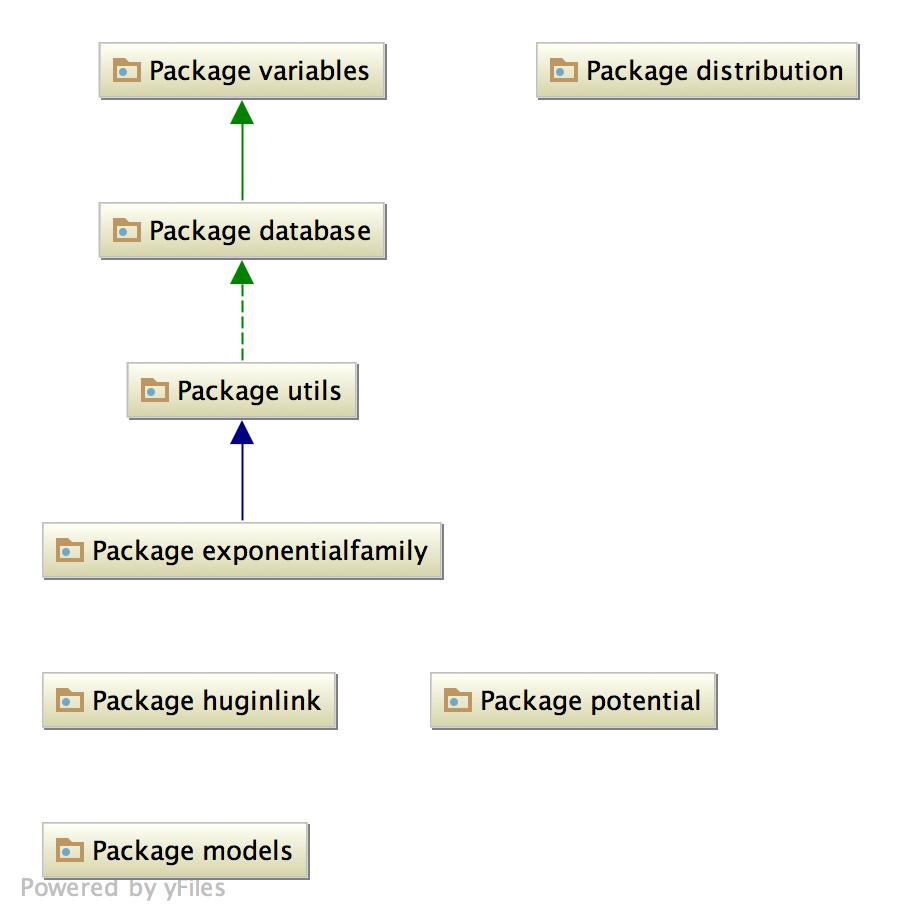
\includegraphics[width=0.5\textwidth]{ClassDiagrams/core.jpg}
\end{figure}

%---------------------------------------------------------------------------------------------------------------
\subsection{Package eu.amidst.core.database}
%---------------------------------------------------------------------------------------------------------------
\begin{figure}[H]
  \centering
    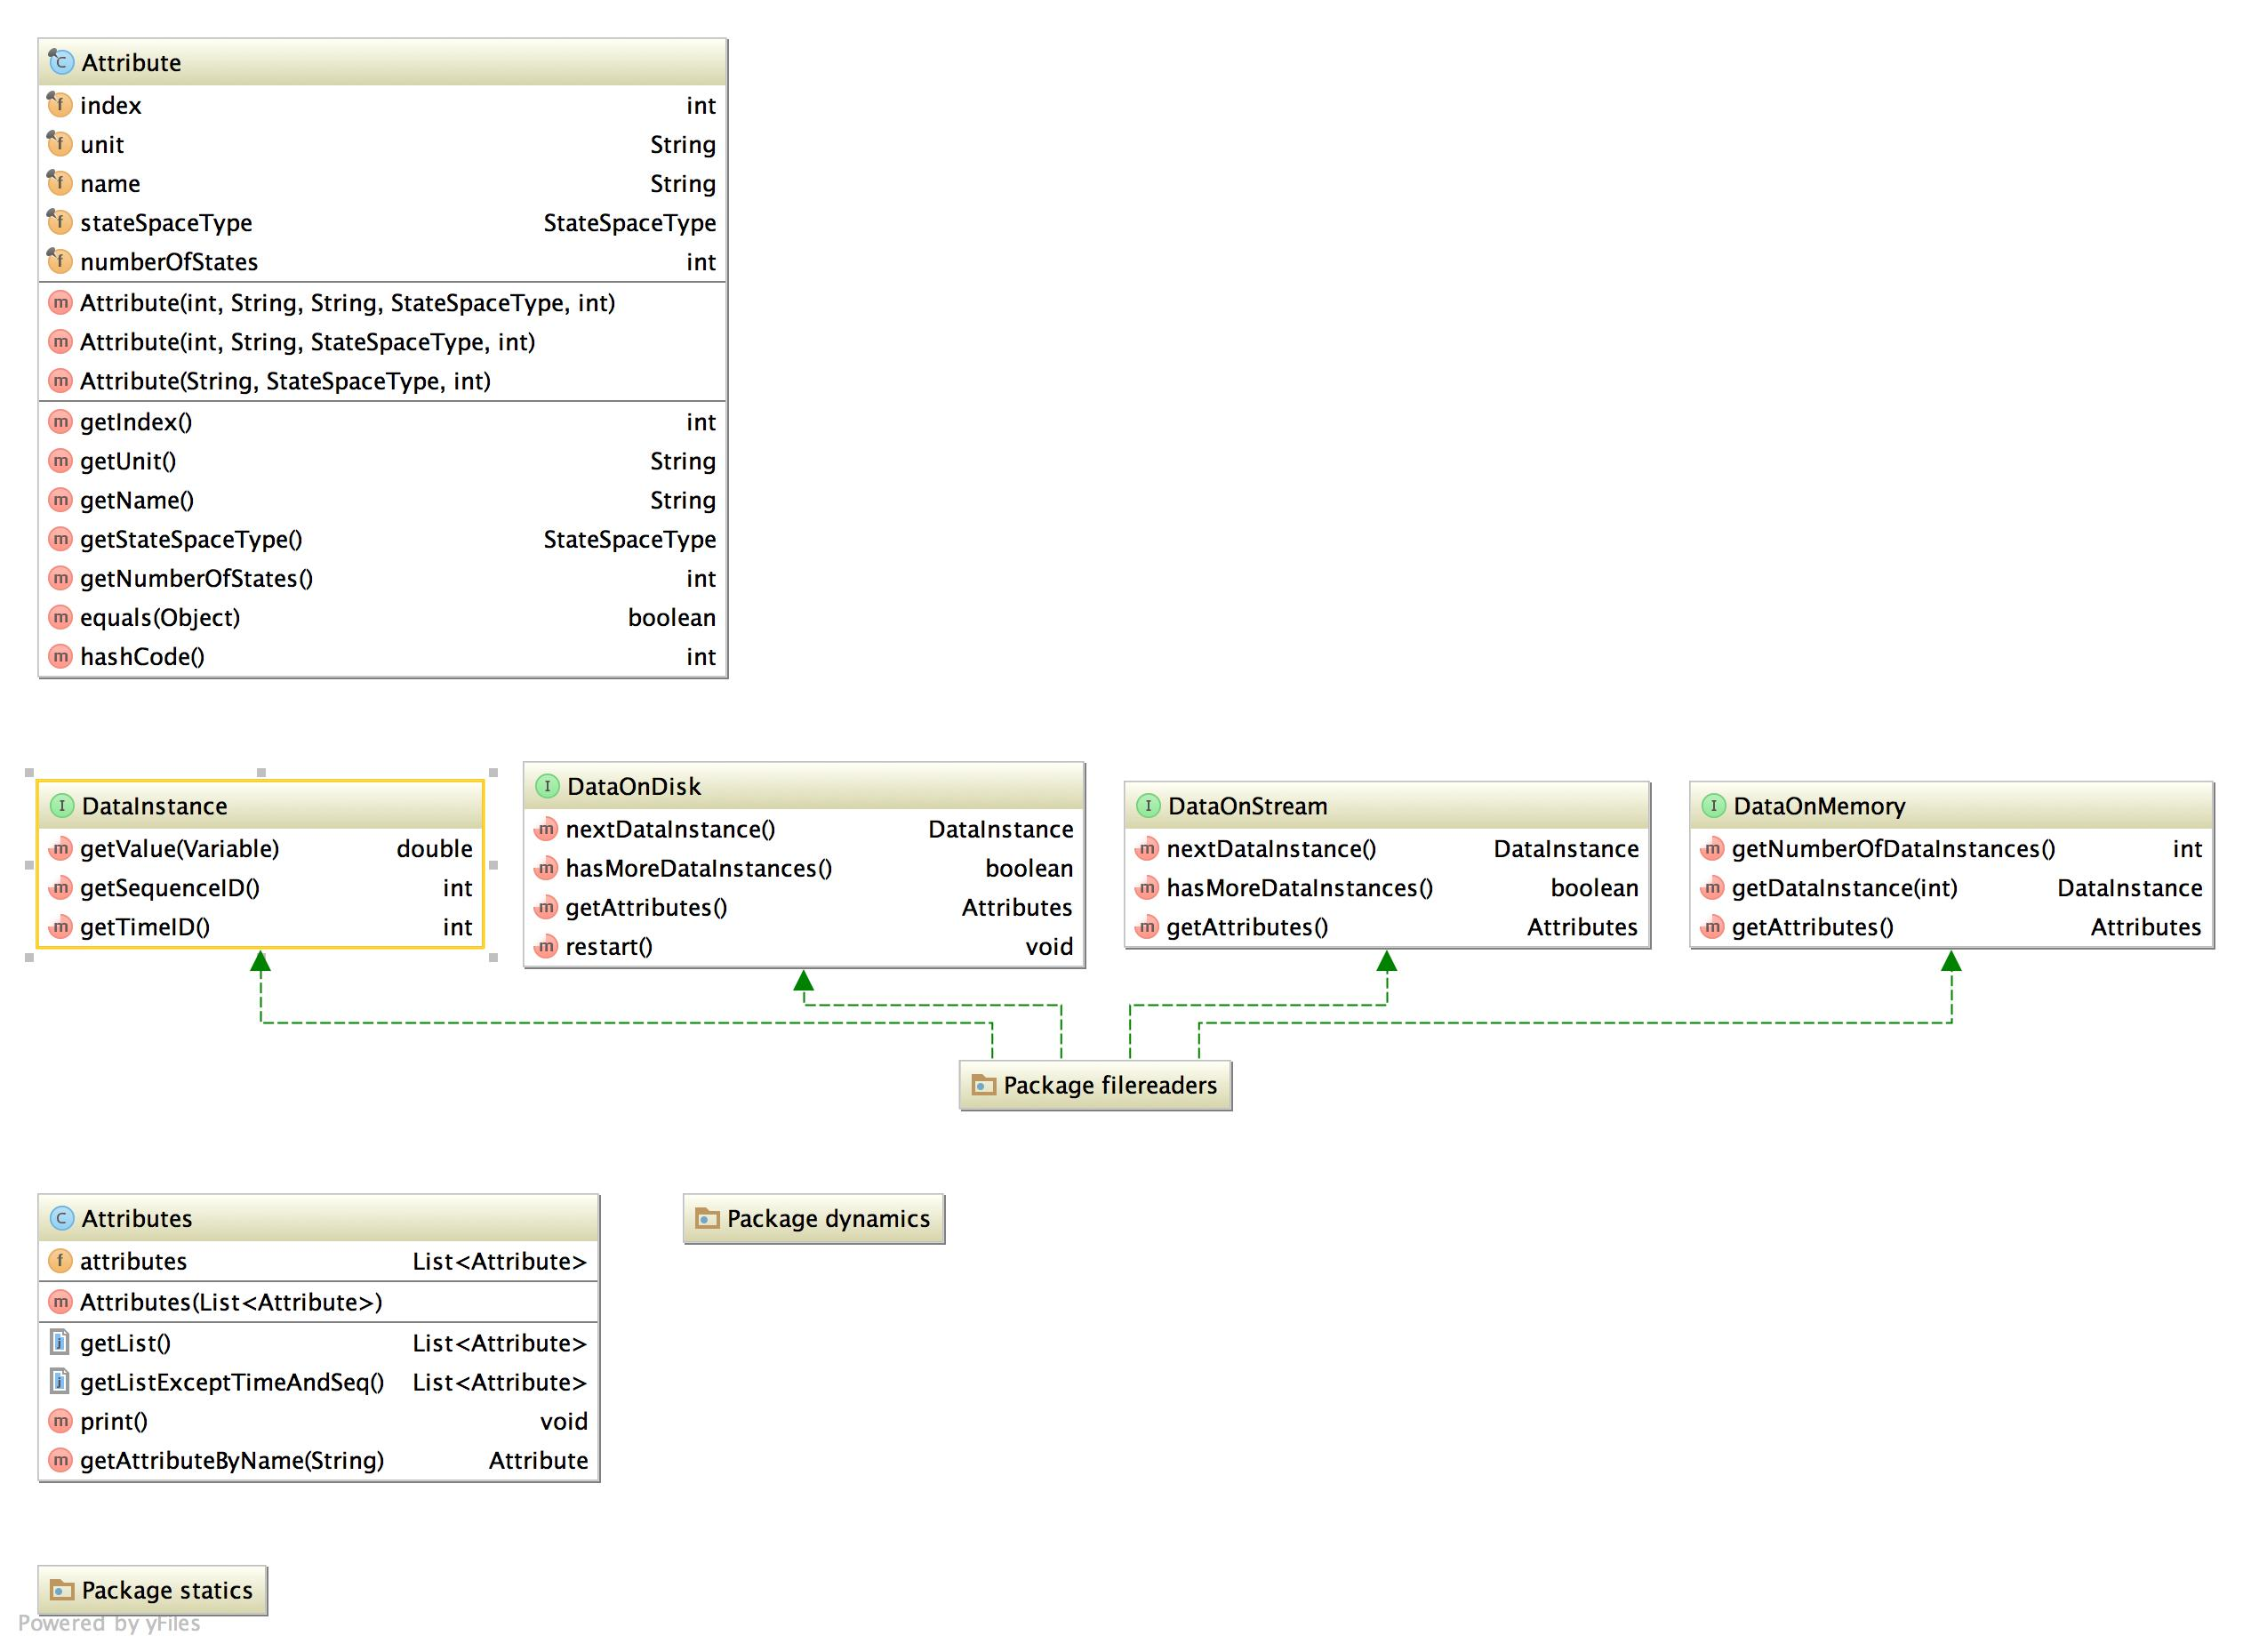
\includegraphics[width=\textwidth]{ClassDiagrams/core_database.jpg}
\end{figure}


%---------------------------------------------------------------------------------------------------------------
\subsection{Package eu.amidst.core.database.dynamics}
%---------------------------------------------------------------------------------------------------------------
\begin{figure}[H]
  \centering
    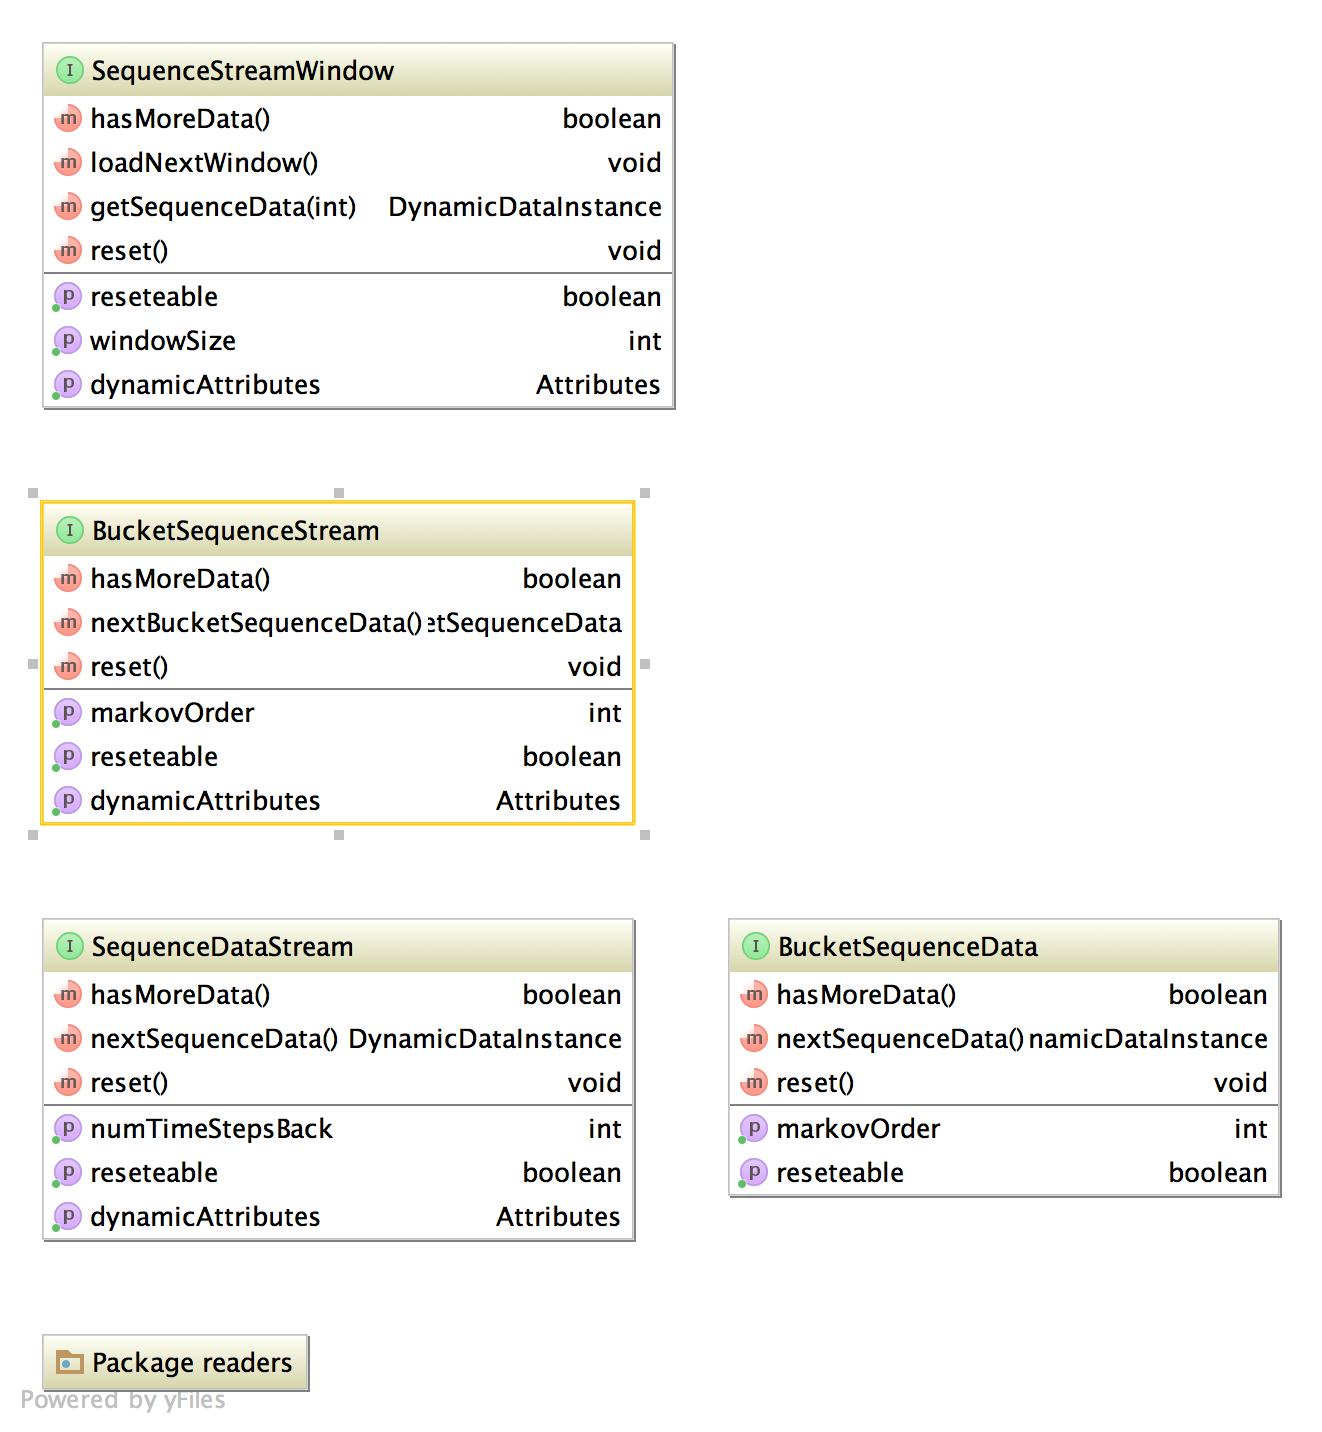
\includegraphics[width=0.7\textwidth]{ClassDiagrams/core_database_dynamics.jpg}
\end{figure}


%---------------------------------------------------------------------------------------------------------------
\subsection{Package eu.amidst.core.database.readers}
%---------------------------------------------------------------------------------------------------------------
\begin{figure}[H]
  \centering
    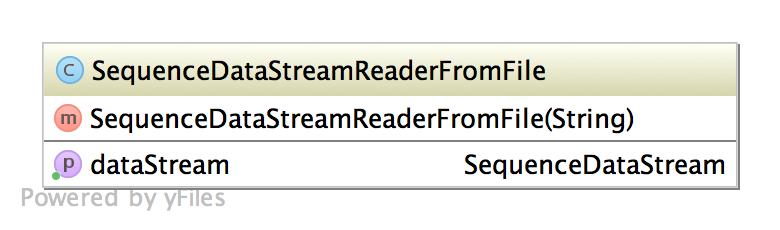
\includegraphics[width=0.4\textwidth]{ClassDiagrams/core_database_dynamics_readers.jpg}
\end{figure}

%---------------------------------------------------------------------------------------------------------------
\subsection{Package eu.amidst.core.database.filereaders}
%---------------------------------------------------------------------------------------------------------------
\begin{figure}[H]
  \centering
    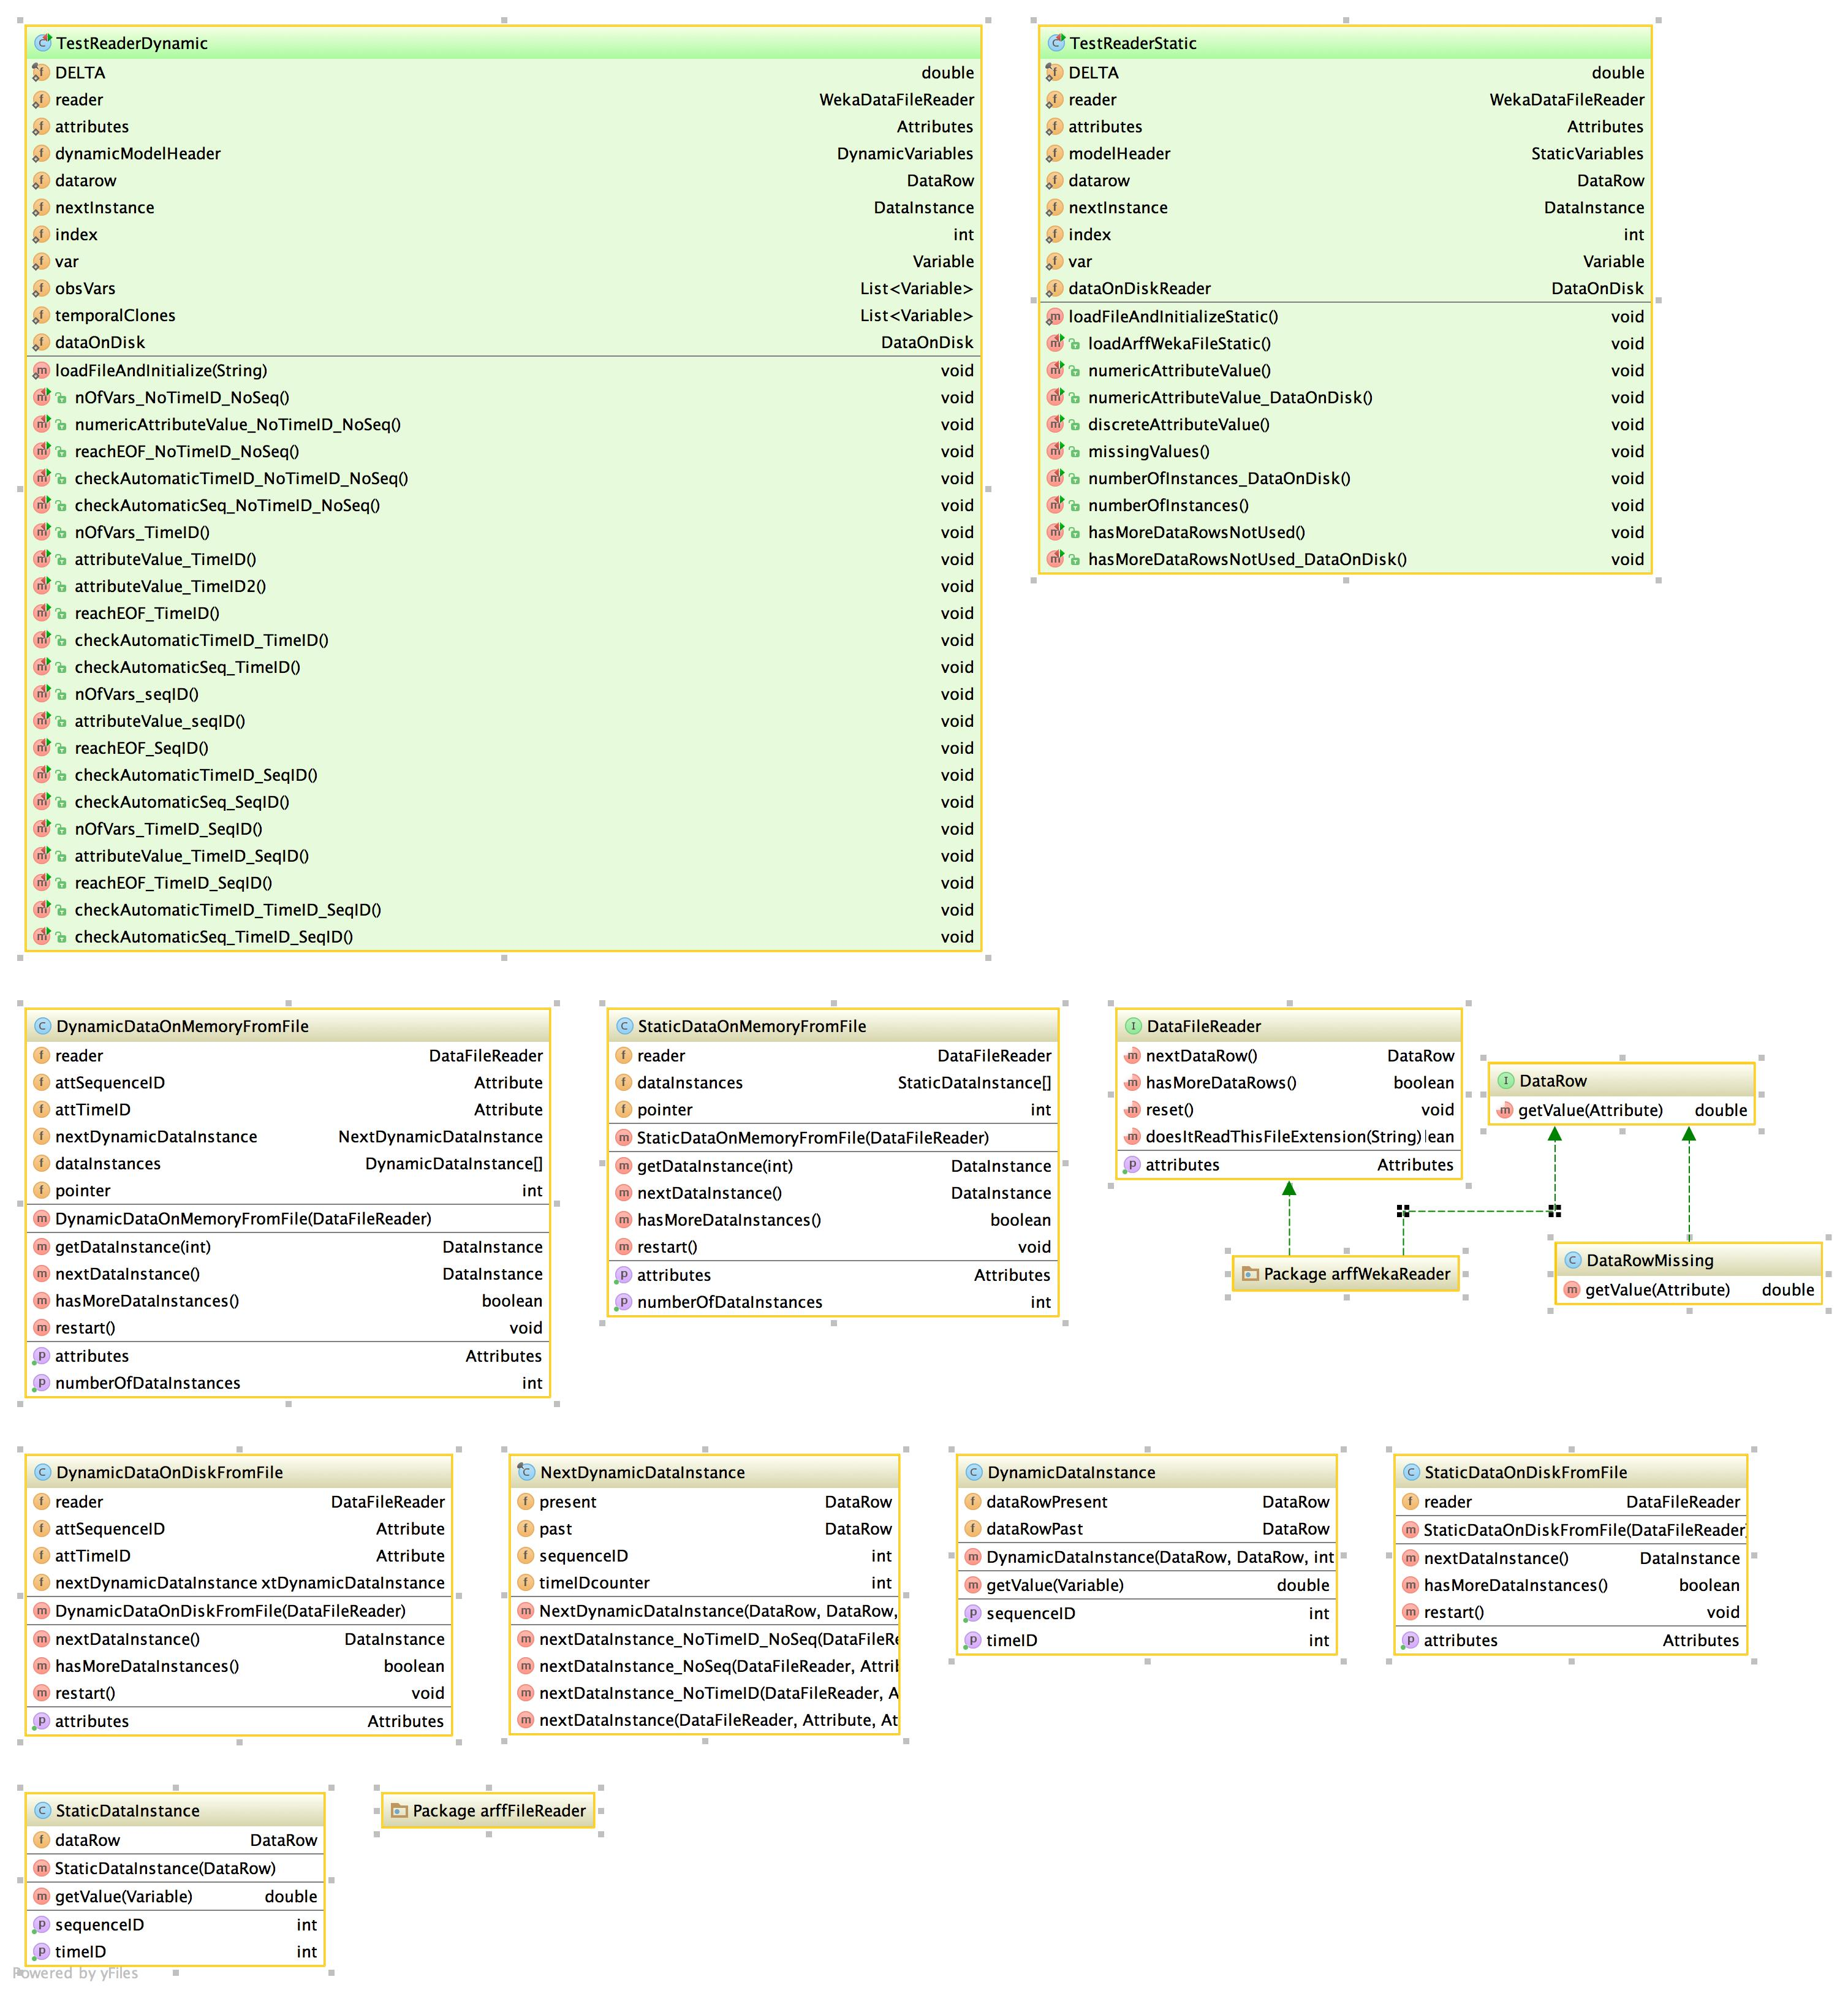
\includegraphics[width=\textwidth]{ClassDiagrams/core_database_filereaders.jpg}
\end{figure}

%---------------------------------------------------------------------------------------------------------------
\subsection{Package eu.amidst.core.database.arffFileReader}
%---------------------------------------------------------------------------------------------------------------

\begin{figure}[H]
  \centering
    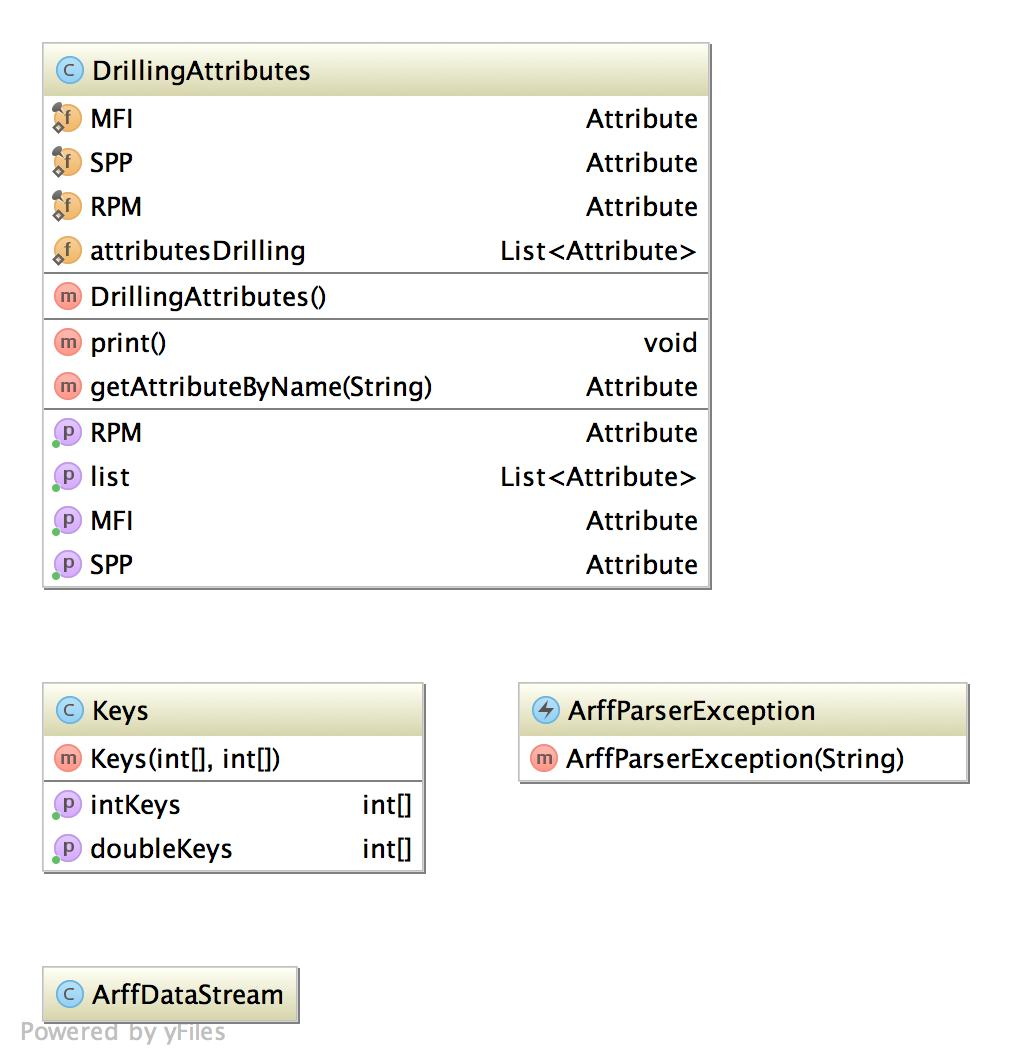
\includegraphics[width=0.5\textwidth]{ClassDiagrams/core_database_filereaders_arfffilereader.jpg}
\end{figure}

%---------------------------------------------------------------------------------------------------------------
\subsection{Package eu.amidst.core.database.arffWekaReader}
%---------------------------------------------------------------------------------------------------------------
\begin{figure}[H]
  \centering
    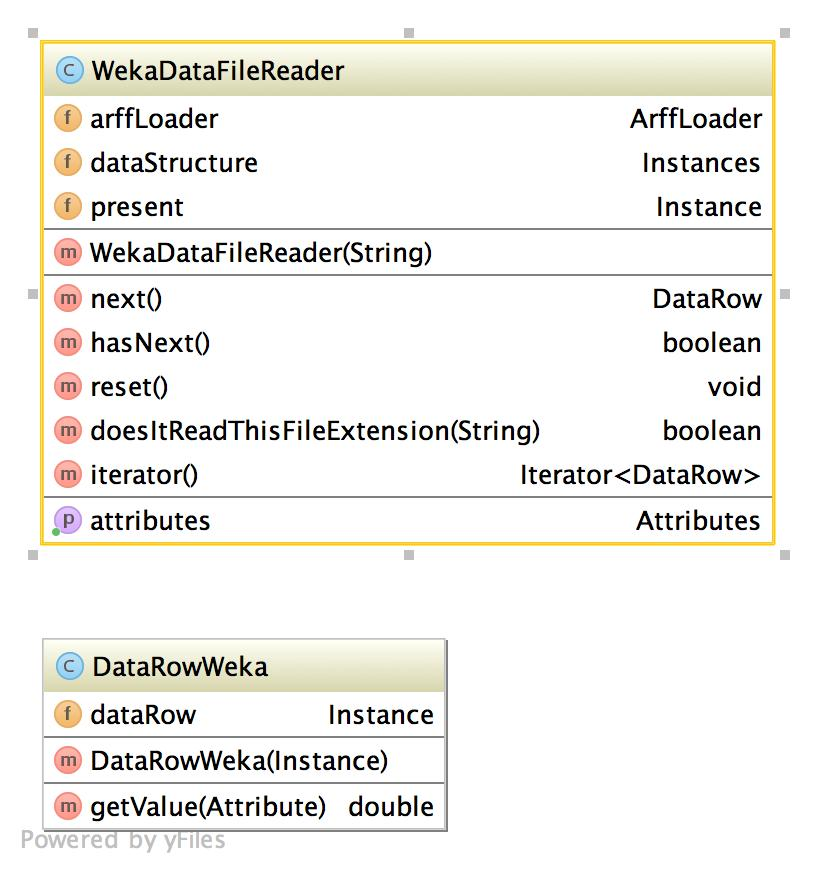
\includegraphics[width=0.5\textwidth]{ClassDiagrams/core_database_filereaders_arffwekareader.jpg}
\end{figure}

%---------------------------------------------------------------------------------------------------------------
\subsection{Package eu.amidst.core.variables}
%---------------------------------------------------------------------------------------------------------------

\begin{figure}[H]
  \caption{Class diagram of the package: \texttt{core.variables}}
  \centering
    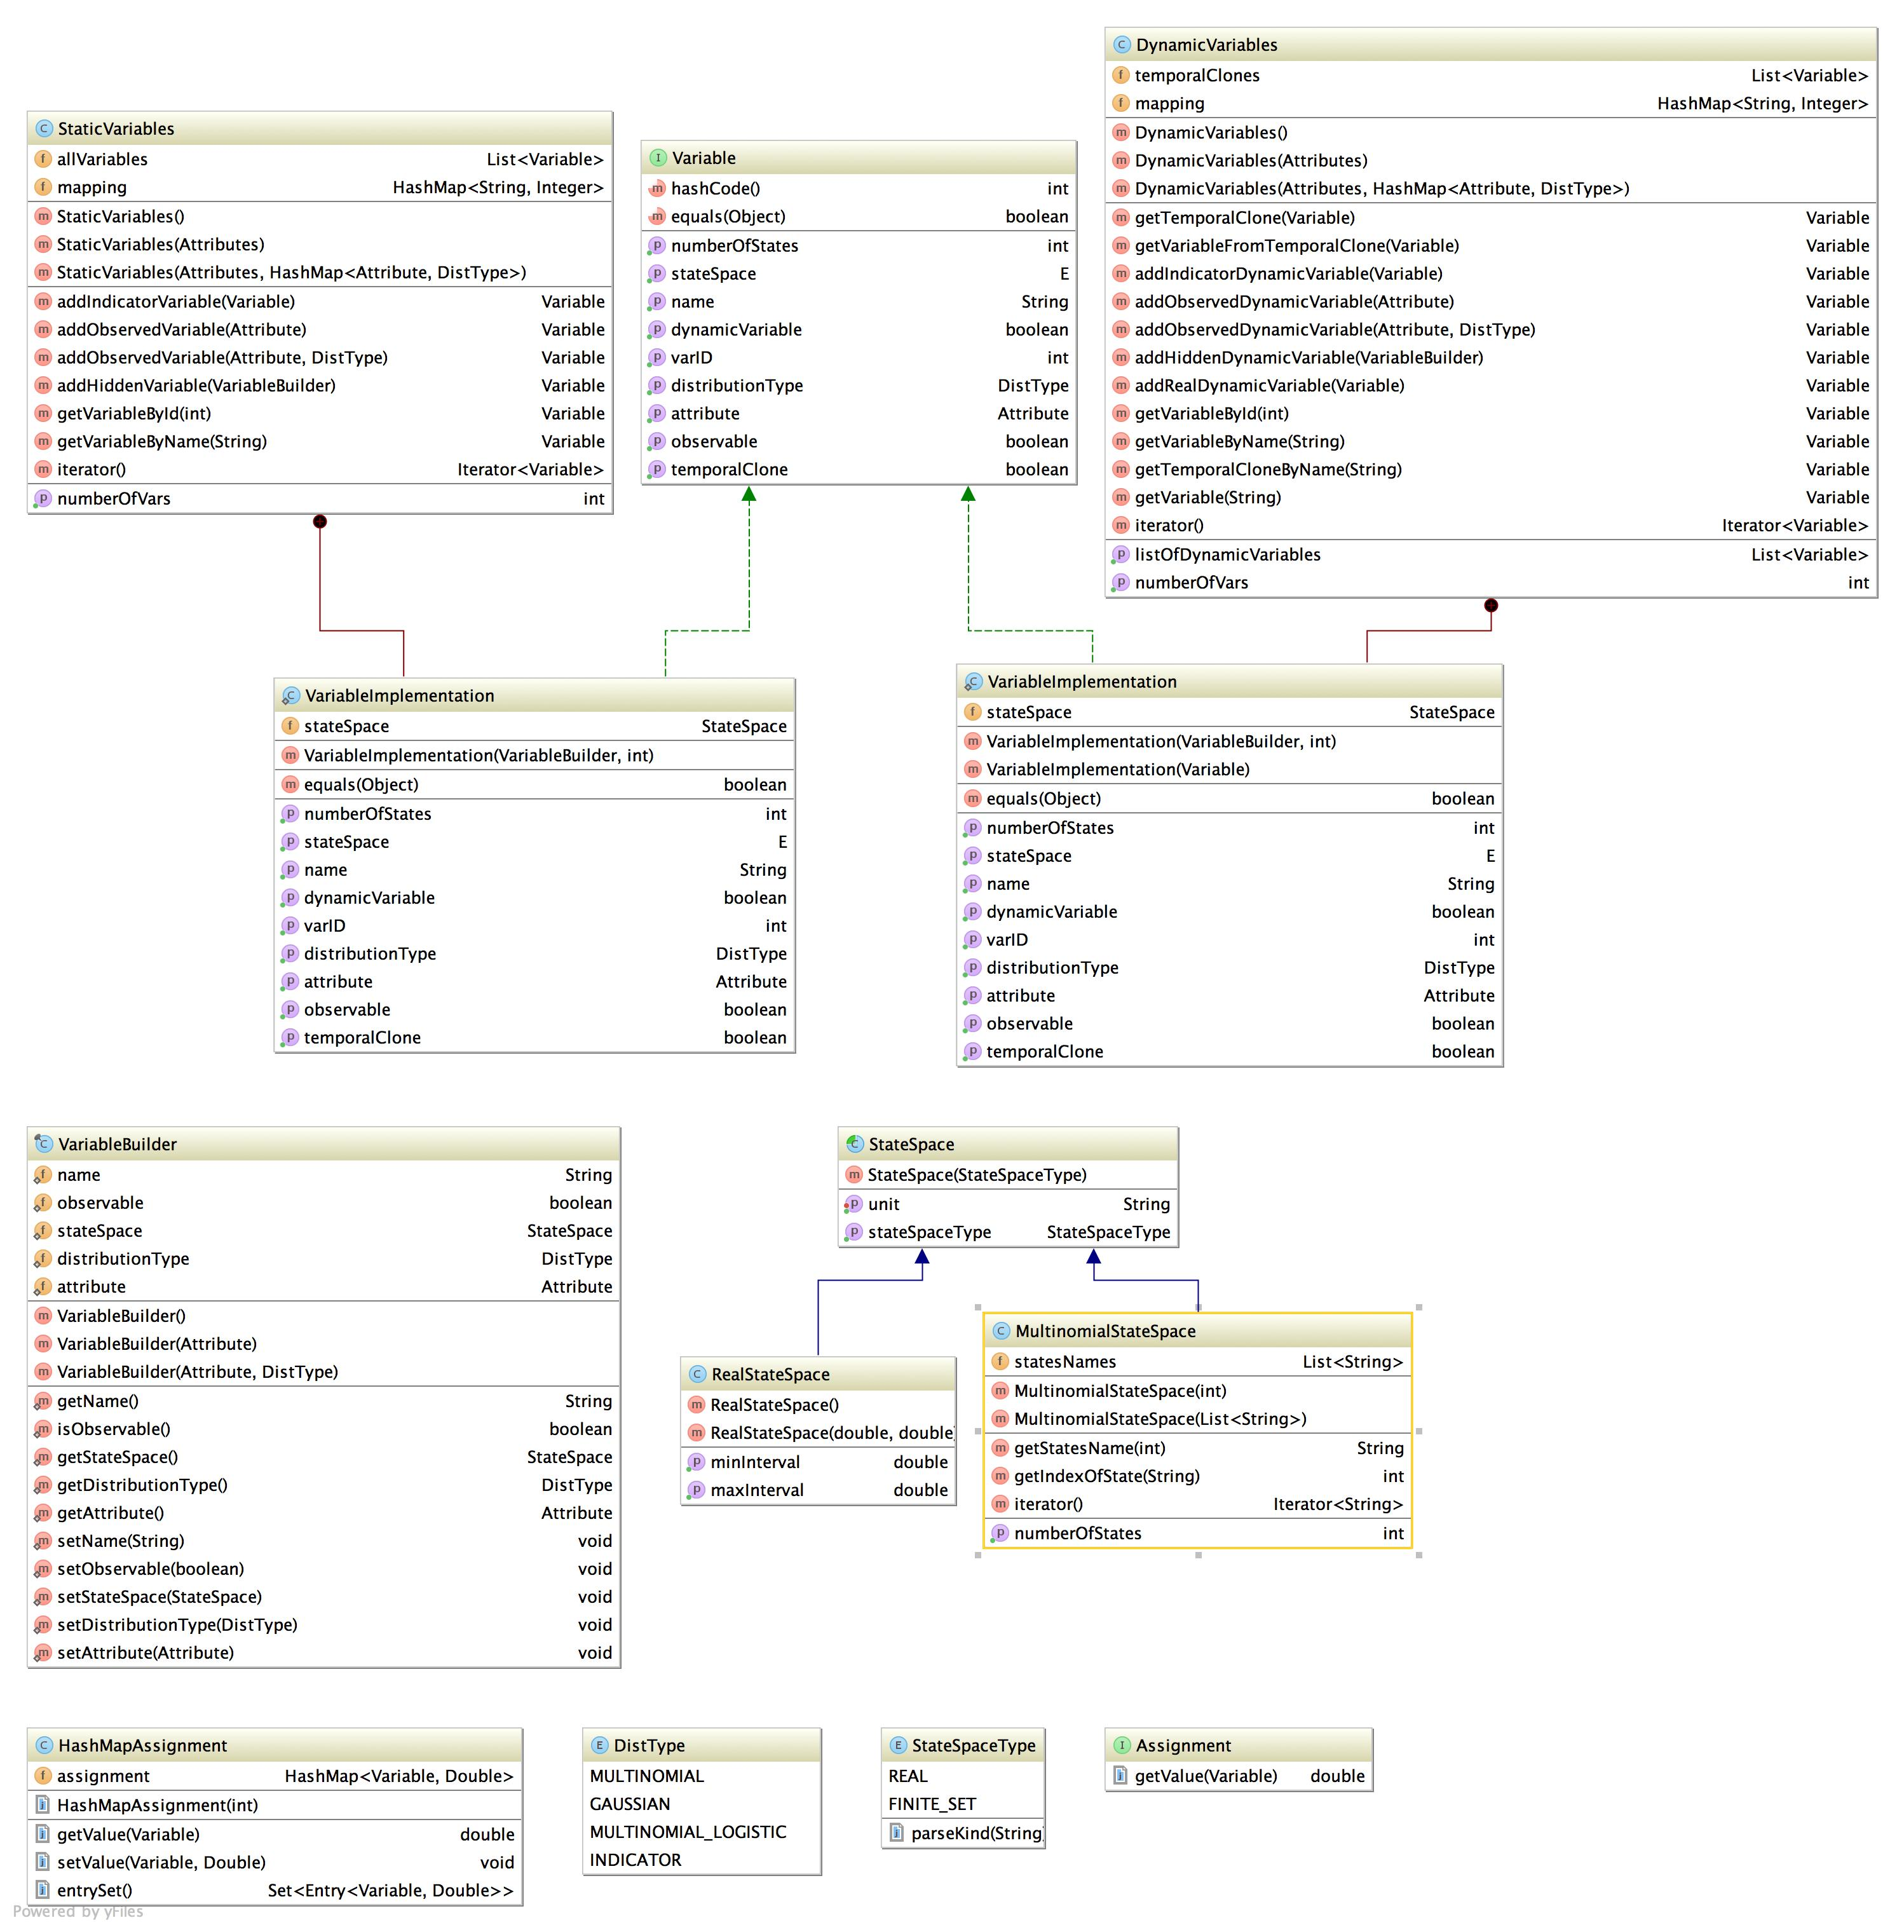
\includegraphics[width=\textwidth]{ClassDiagrams/core_variables.jpg}
\end{figure}

%---------------------------------------------------------------------------------------------------------------
\subsection{Package eu.amidst.core.distribution}
%---------------------------------------------------------------------------------------------------------------

\begin{figure}[H]
  \centering
    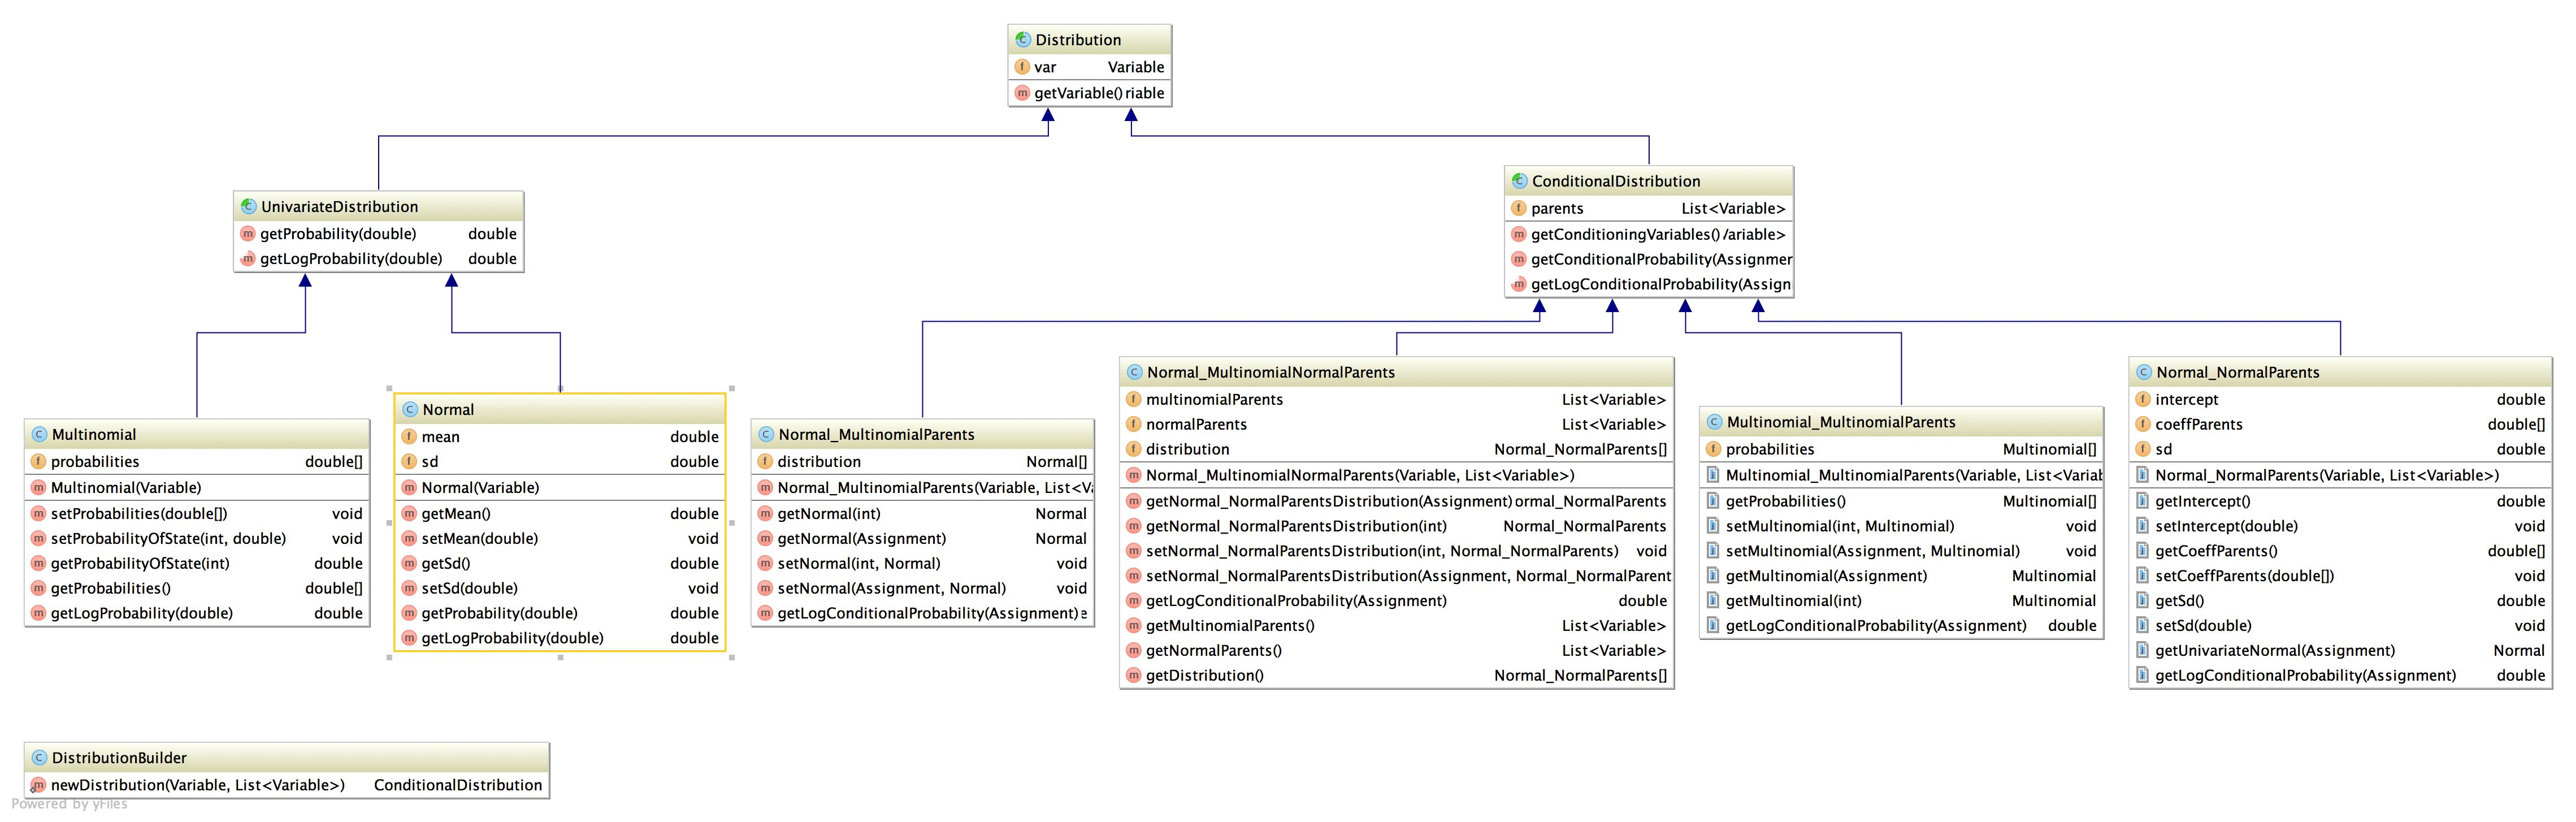
\includegraphics[width=\textwidth]{ClassDiagrams/core_distribution.jpg}
\end{figure}



%---------------------------------------------------------------------------------------------------------------
\subsection{Package eu.amidst.core.models}
%---------------------------------------------------------------------------------------------------------------
\begin{figure}[H]
  \centering
    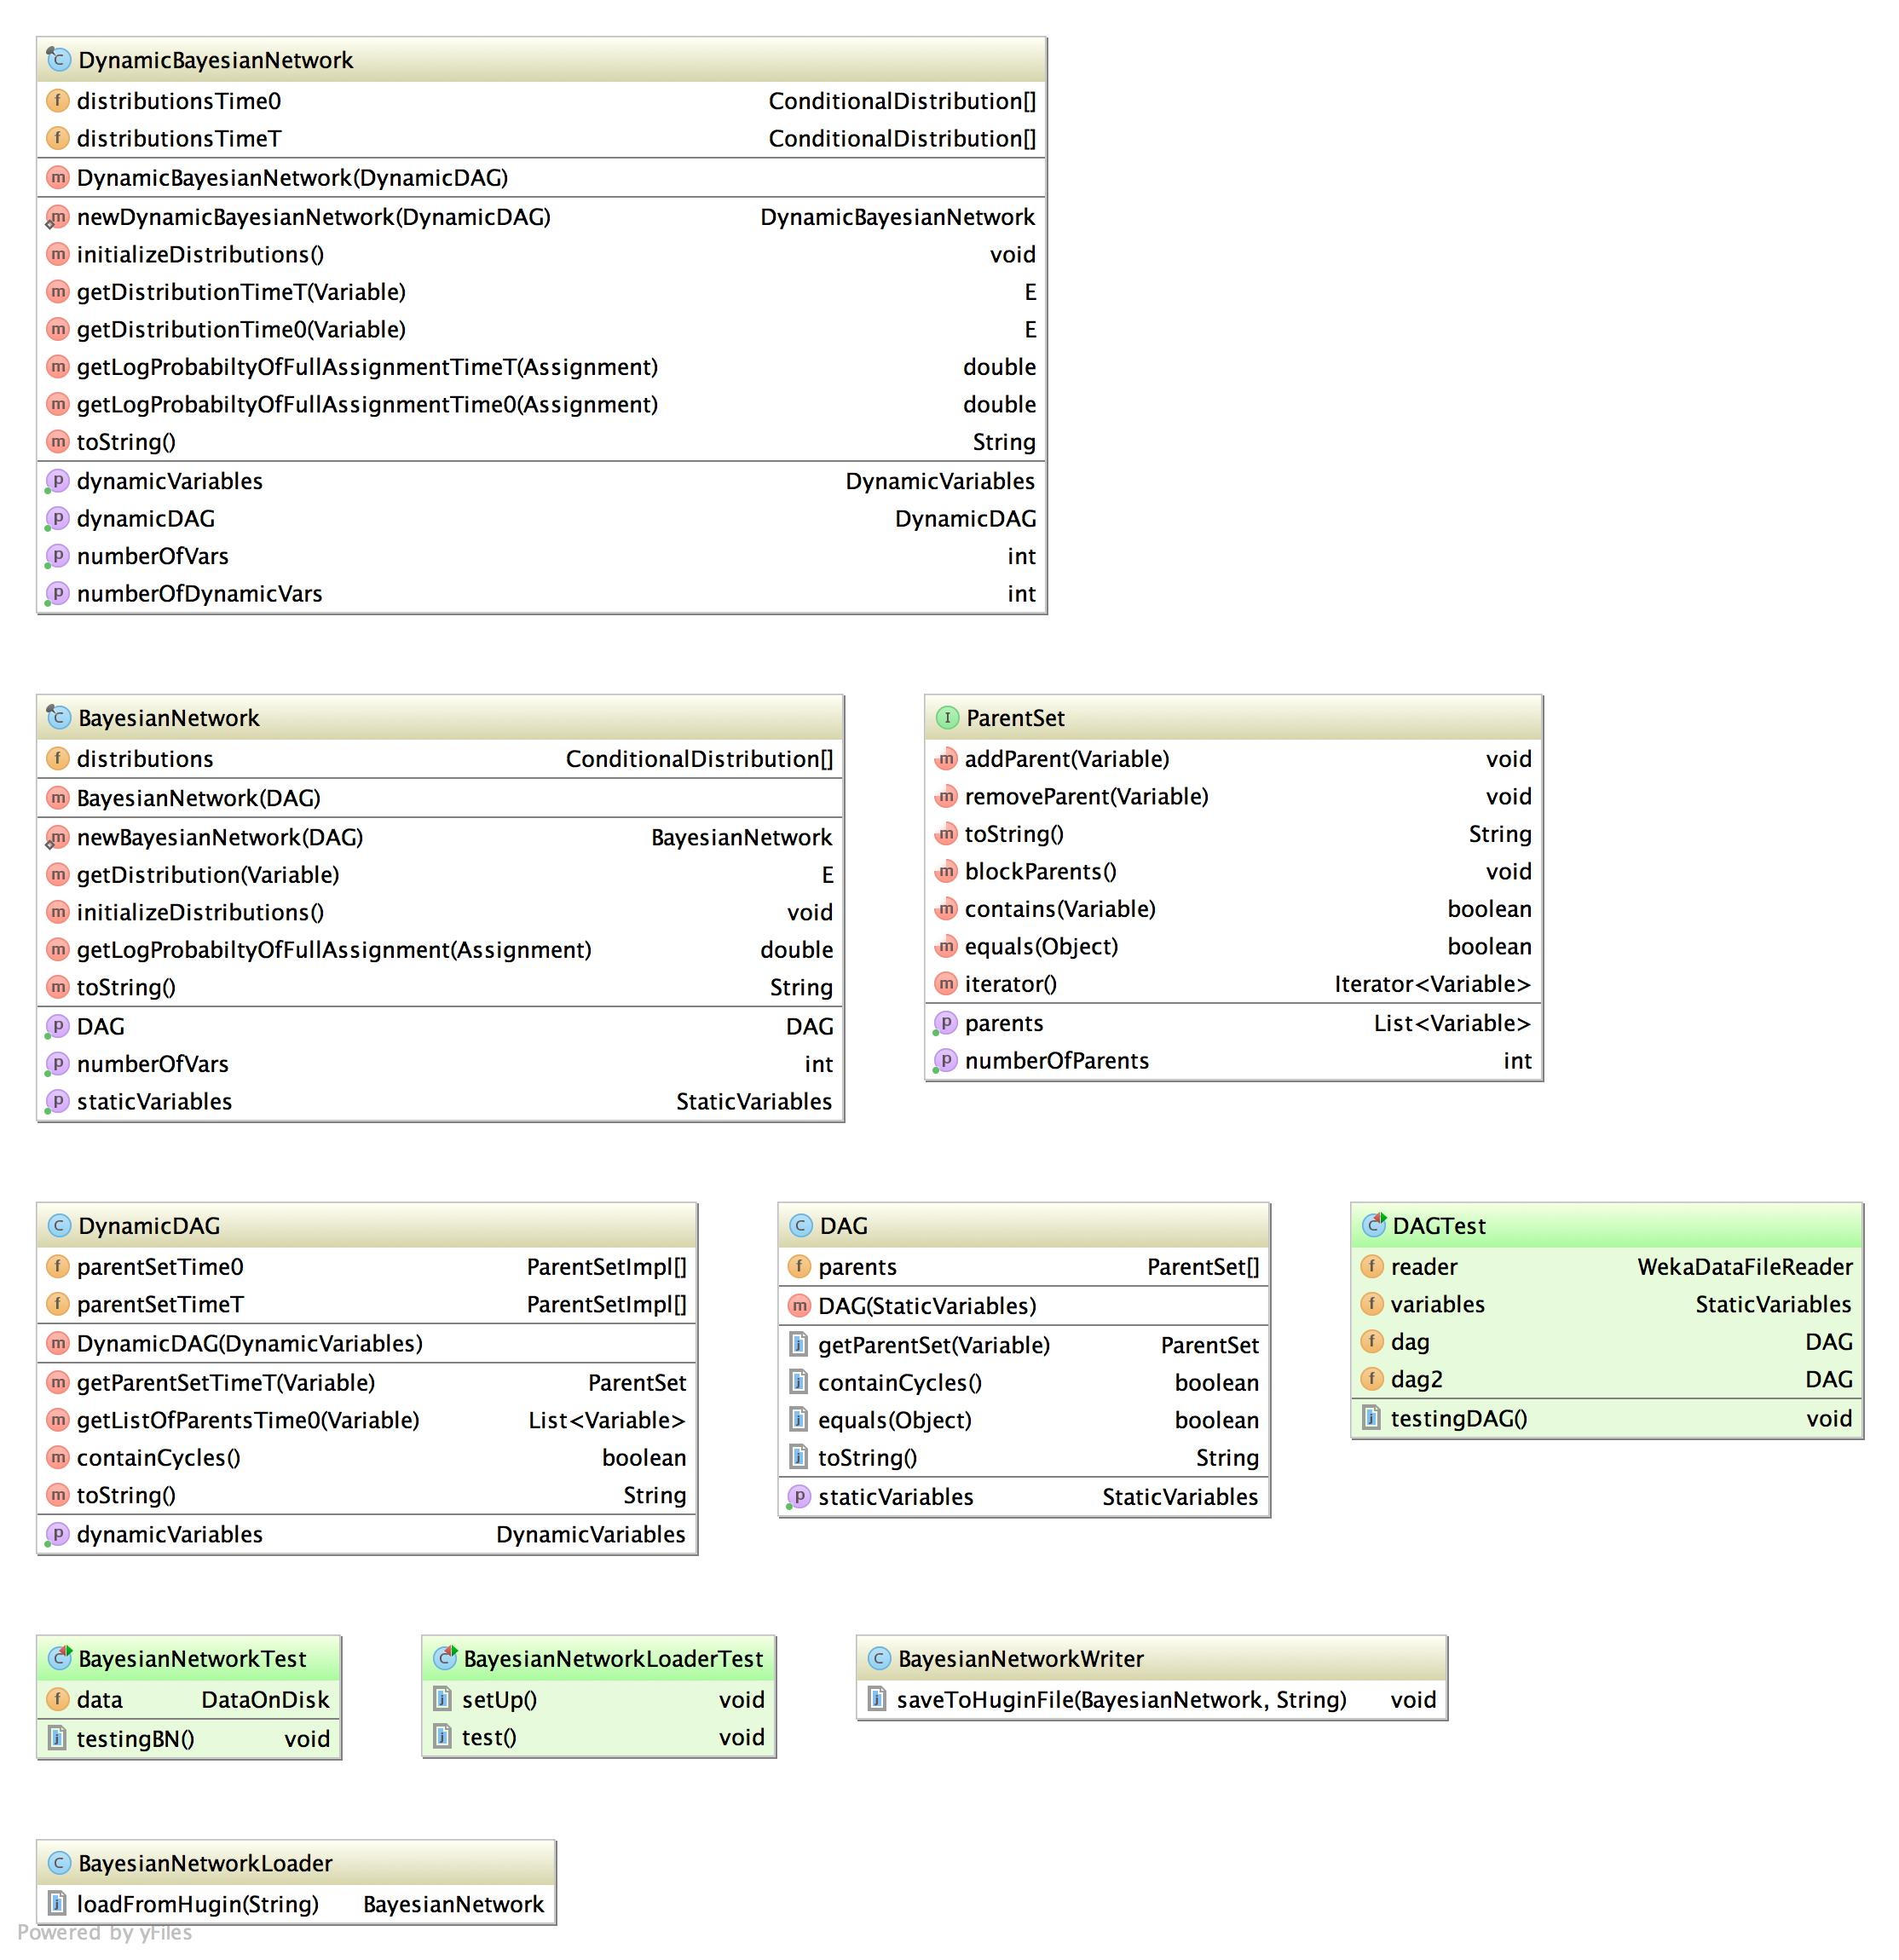
\includegraphics[width=\textwidth]{ClassDiagrams/core_models.jpg}
\end{figure}

%---------------------------------------------------------------------------------------------------------------
\subsection{Package eu.amidst.core.huginlink}
%---------------------------------------------------------------------------------------------------------------

\begin{figure}[H]
  \centering
    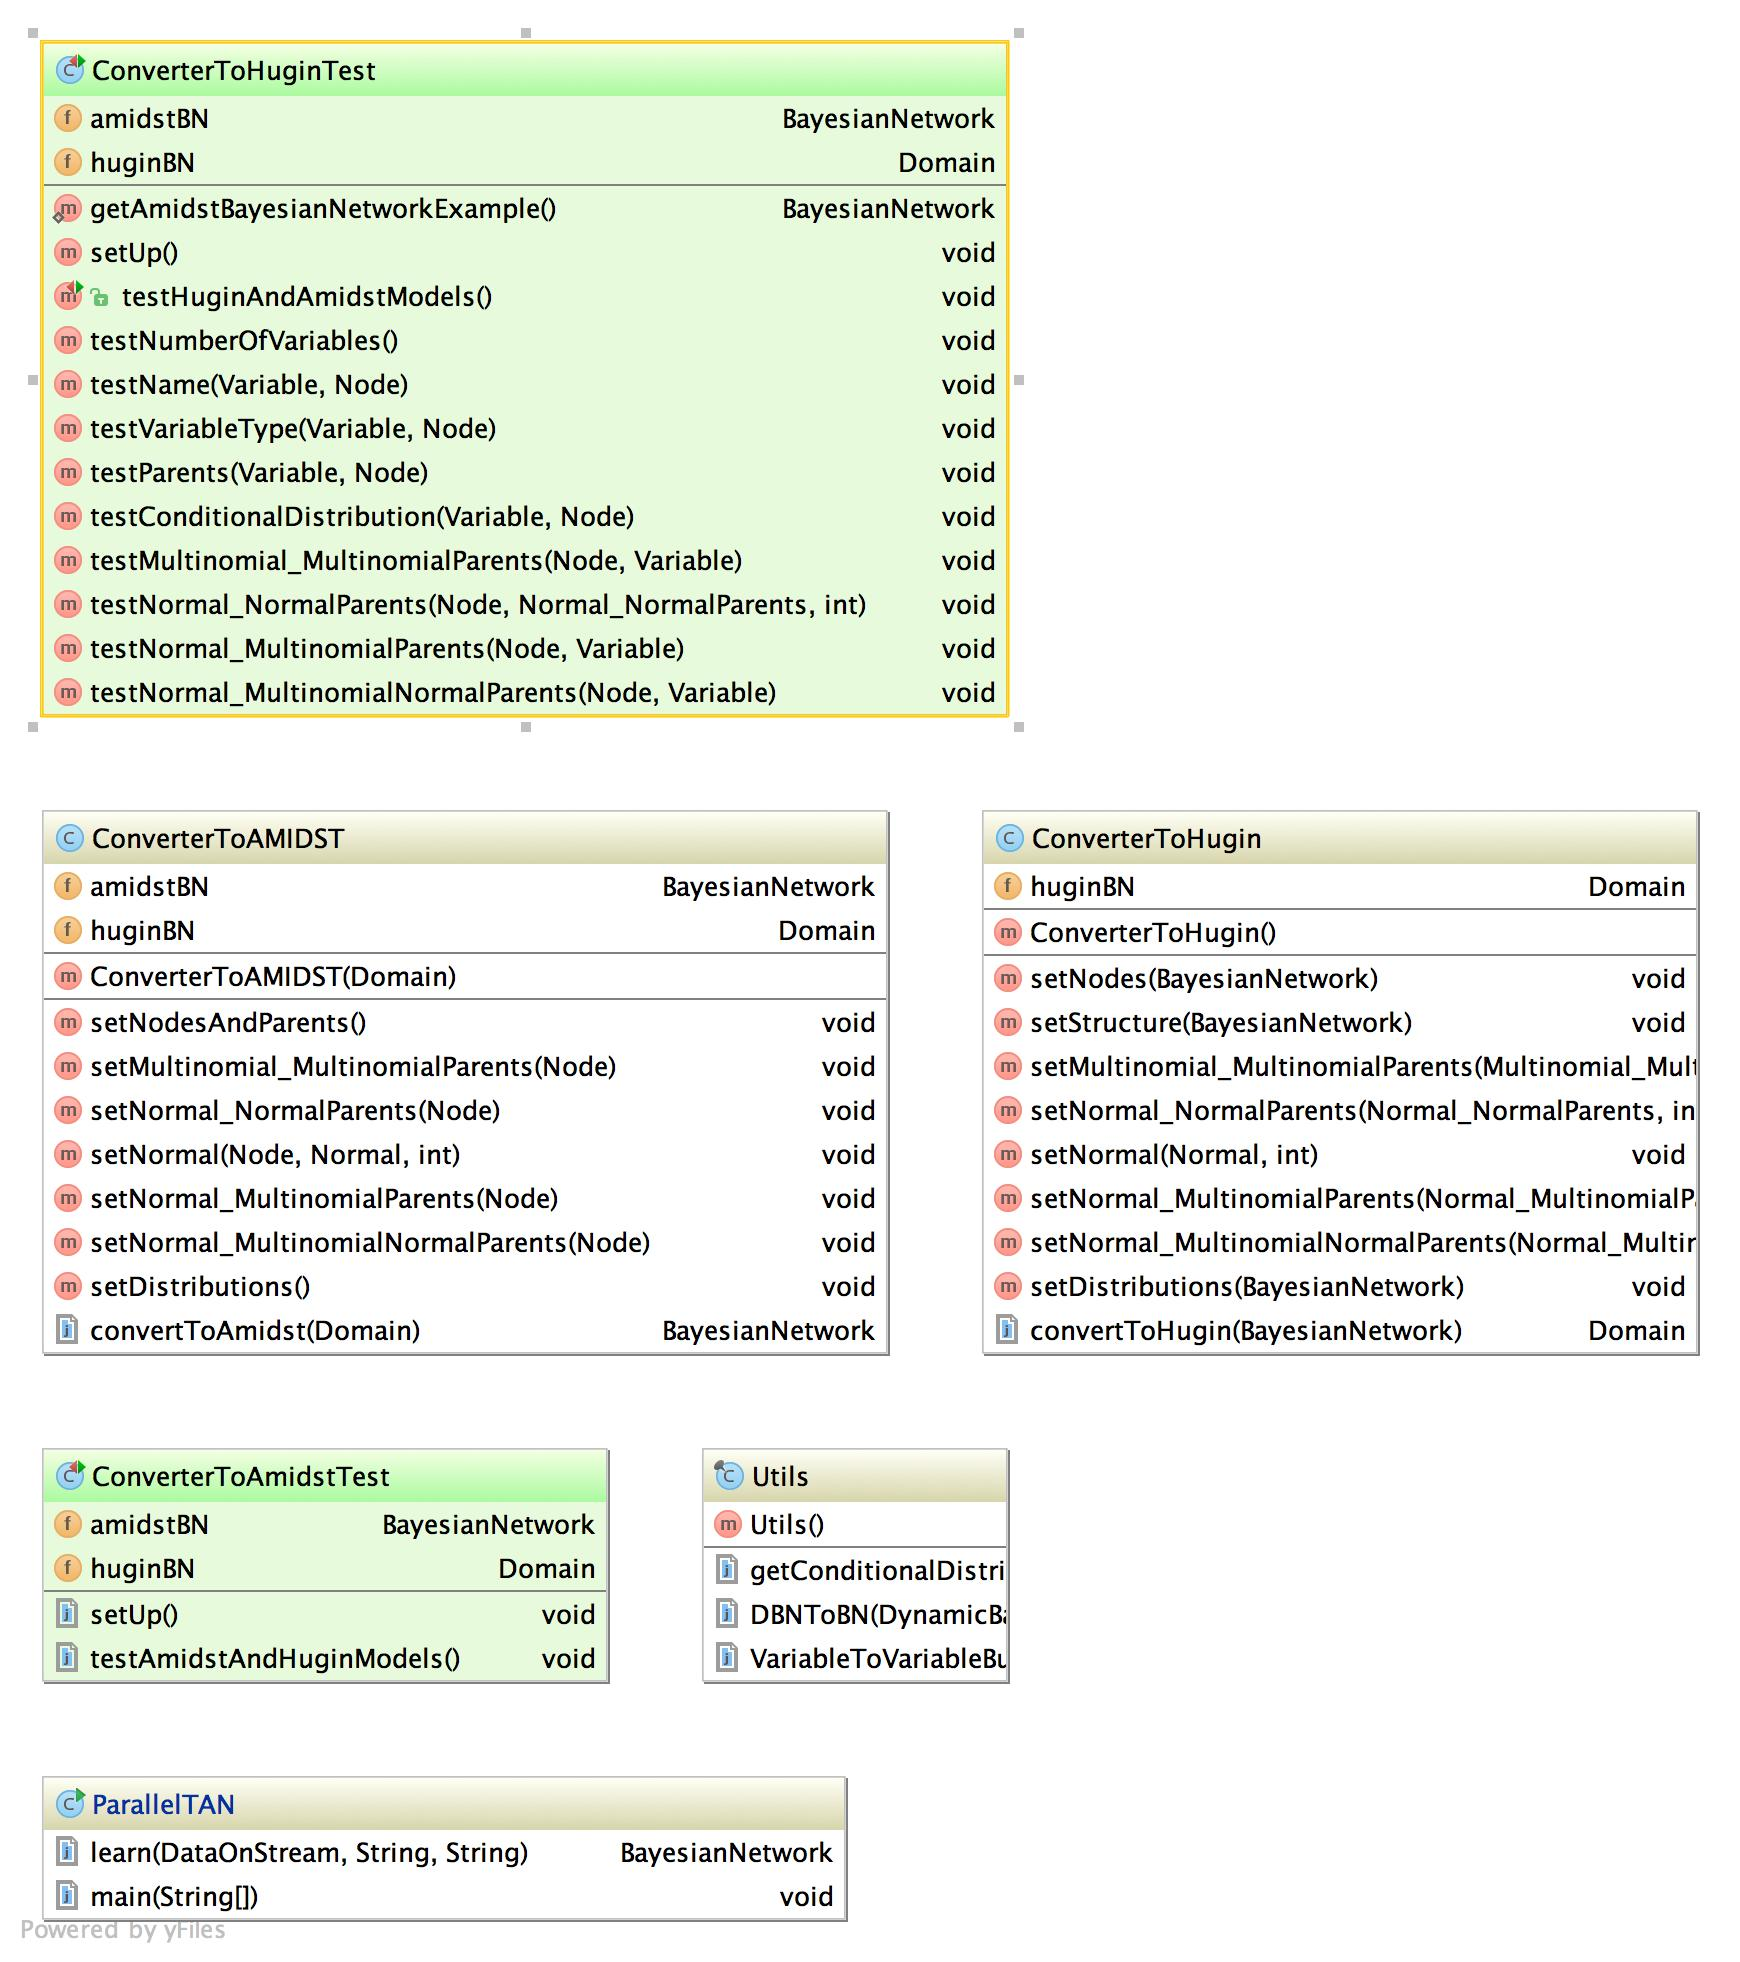
\includegraphics[width=0.7\textwidth]{ClassDiagrams/core_huginlink.jpg}
\end{figure}


%---------------------------------------------------------------------------------------------------------------
\subsection{Package eu.amidst.core.potential}
%---------------------------------------------------------------------------------------------------------------

\begin{figure}[H]
  \caption{Class diagram of the package: \texttt{core.potential}}
  \centering
    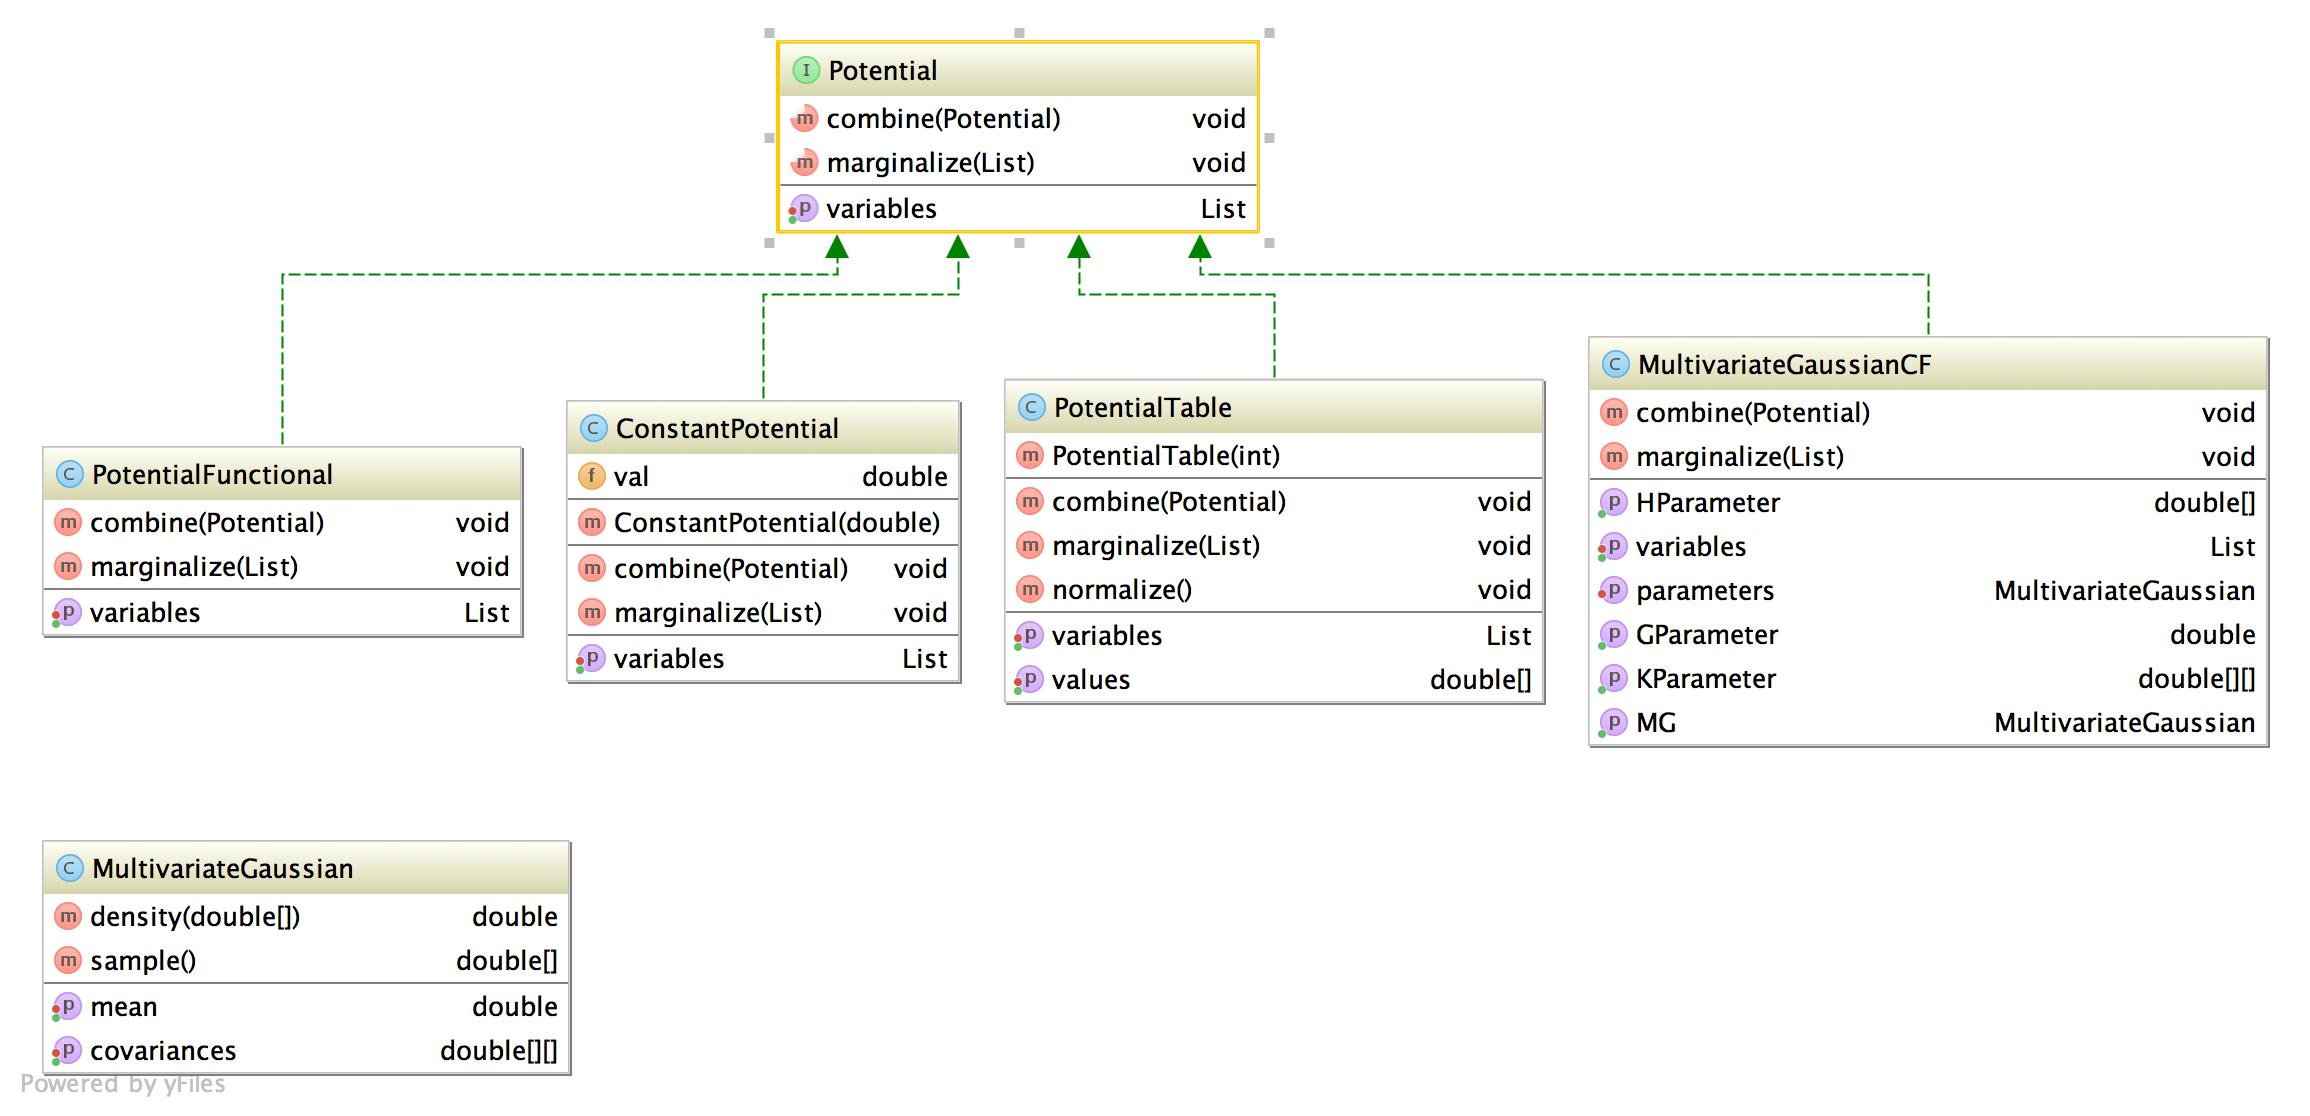
\includegraphics[width=\textwidth]{ClassDiagrams/core_potential.jpg}
\end{figure}

%---------------------------------------------------------------------------------------------------------------
\subsection{Package eu.amidst.core.exponentialfamily}
%---------------------------------------------------------------------------------------------------------------

\begin{figure}[H]
  \centering
    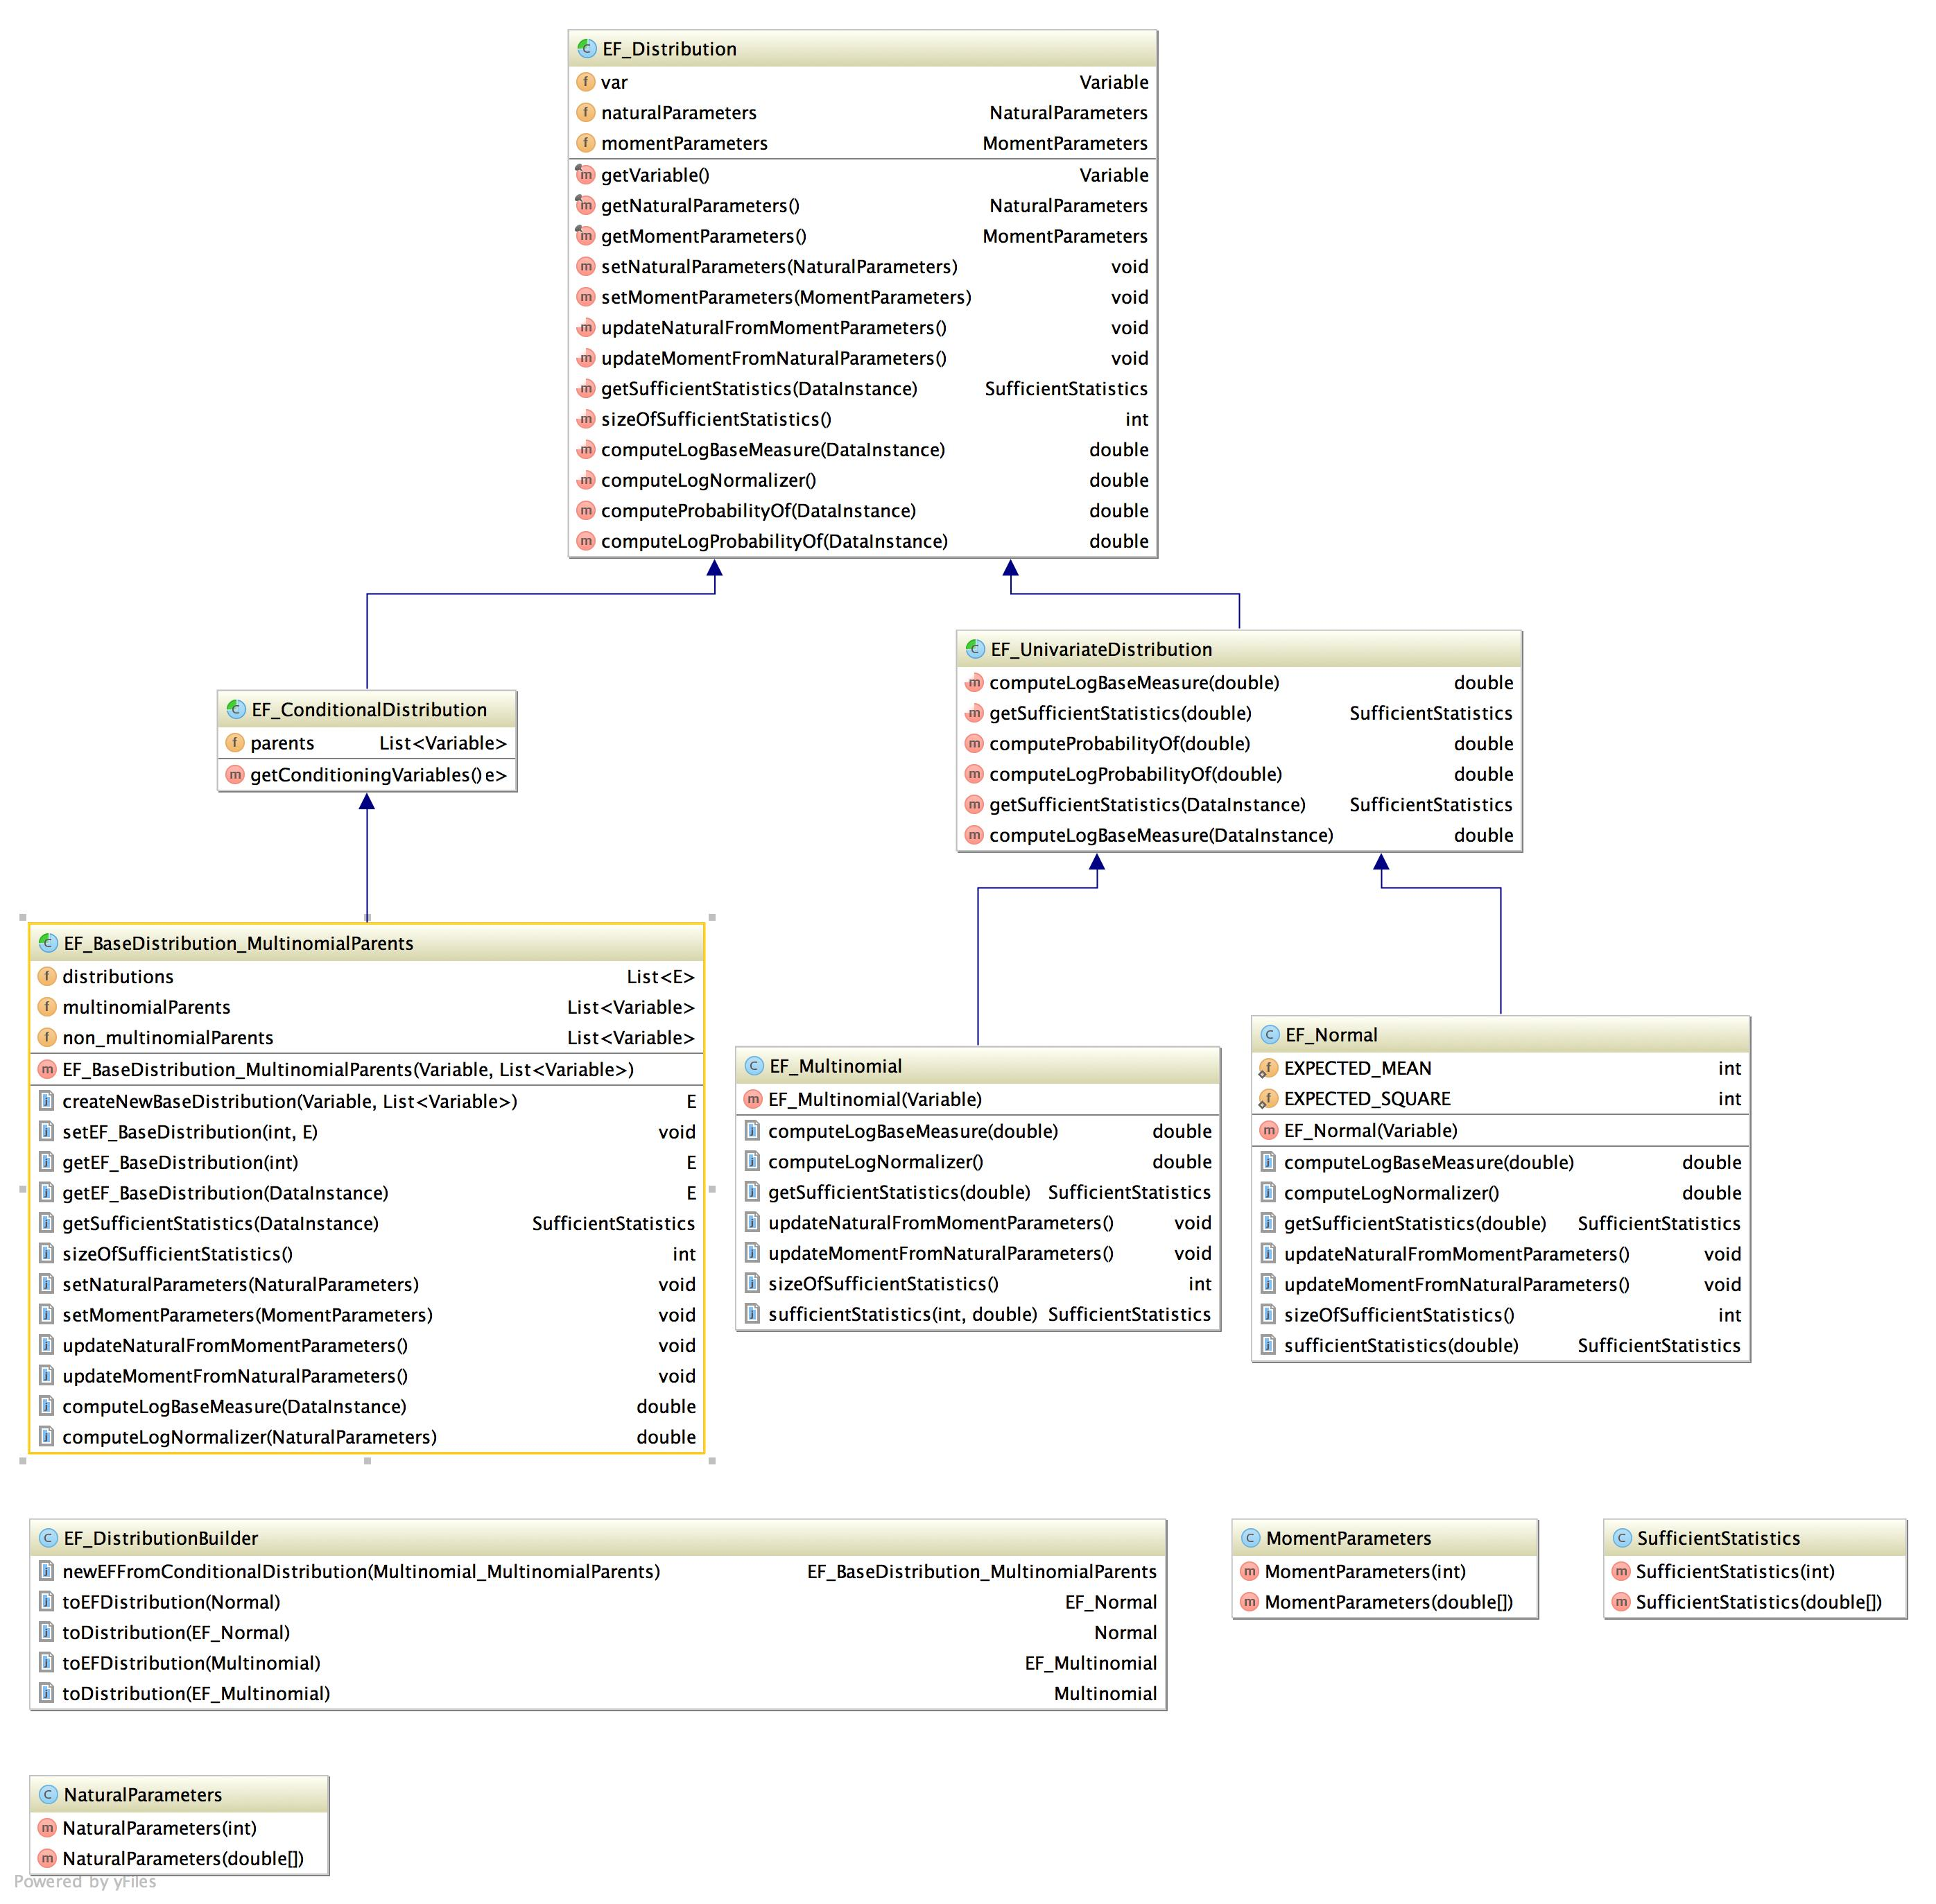
\includegraphics[width=\textwidth]{ClassDiagrams/core_exponentialfamily.jpg}
\end{figure}

%---------------------------------------------------------------------------------------------------------------
\subsection{Package eu.amidst.core.utils}
%---------------------------------------------------------------------------------------------------------------
\begin{figure}[H]
  \centering
    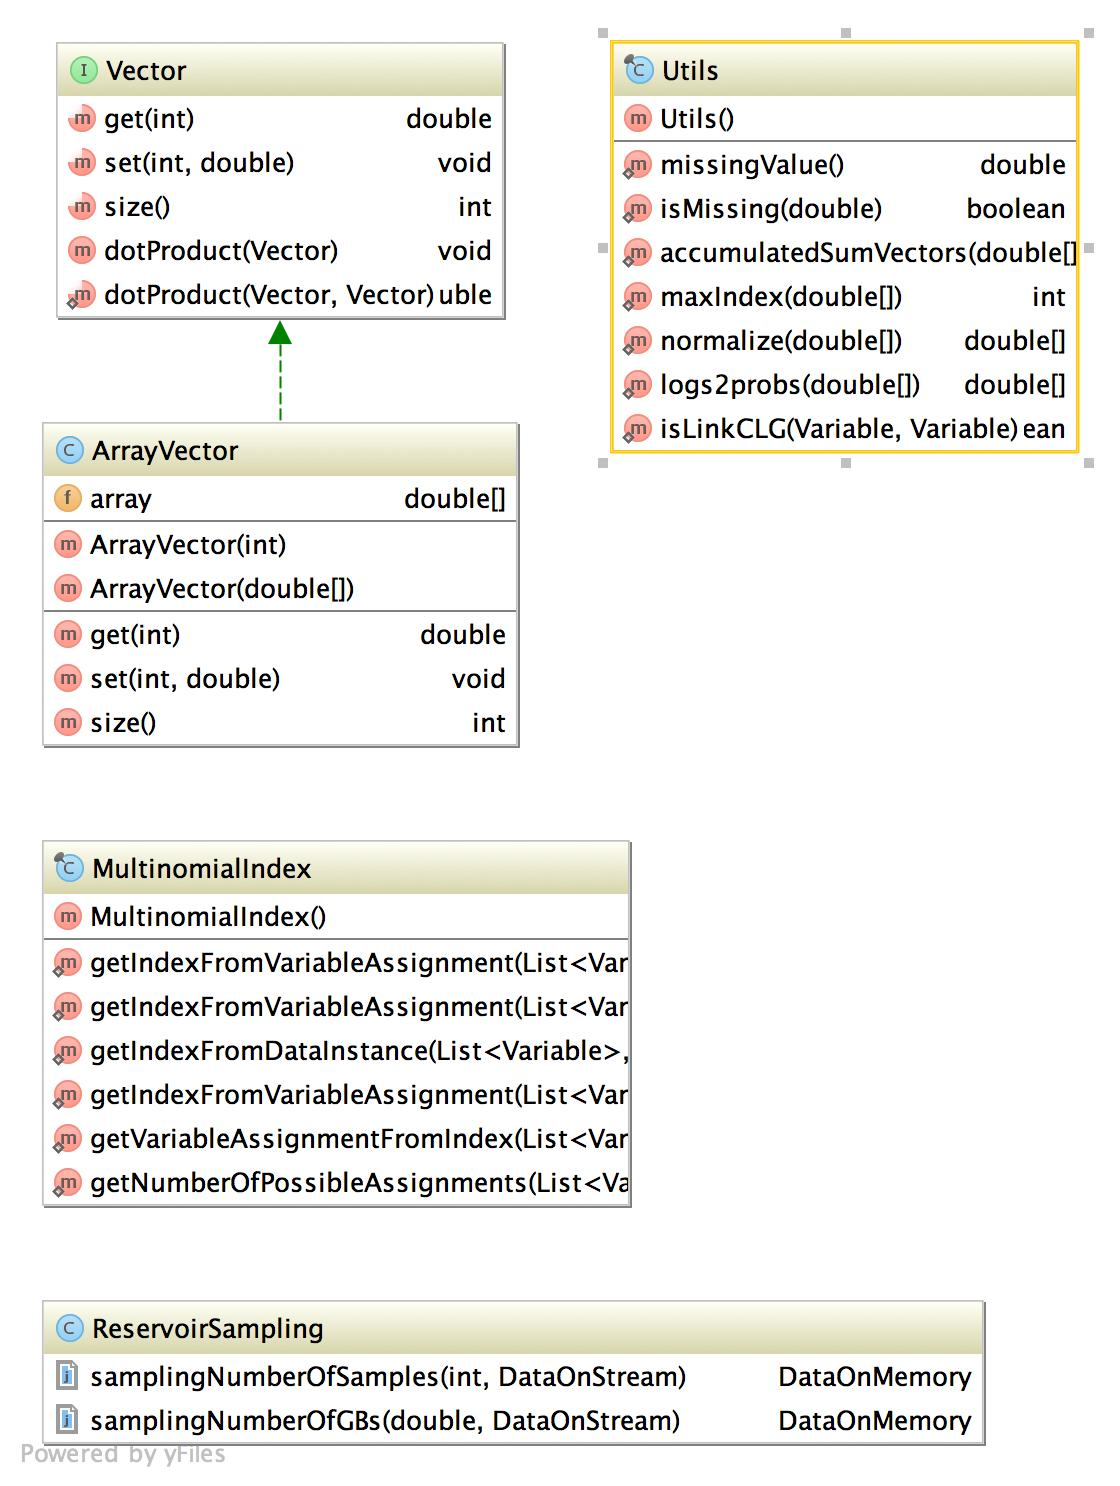
\includegraphics[width=0.6\textwidth]{ClassDiagrams/core_utils.jpg}
\end{figure}
%%%%%%%%%%%%%%%%%%%%%%%%%%%%%%%%%%%%%%%%%



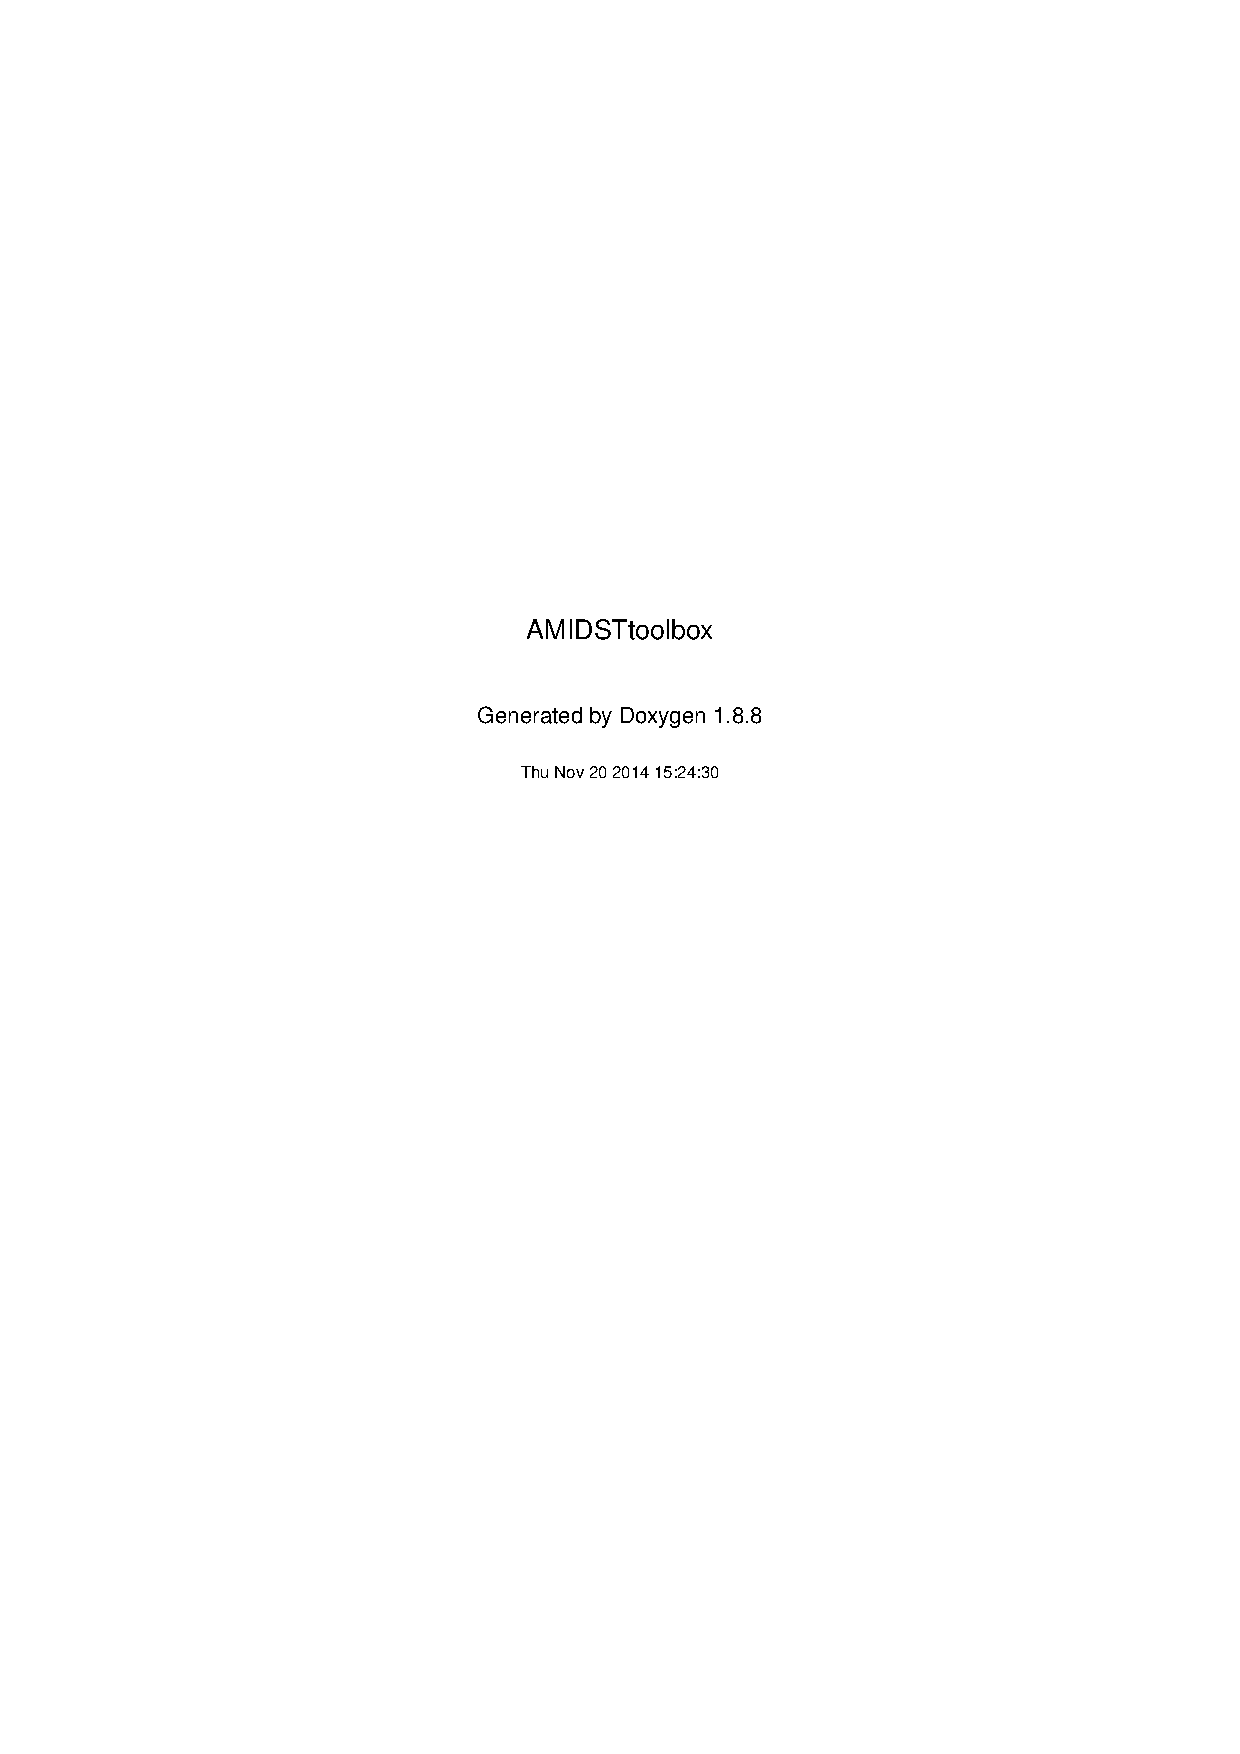
\includepdf{doxygenPDF/refman.pdf}

\bibliographystyle{splncs}
%\bibliography{re}

\appendix
\section{Code Description (Doxygen Document)}
\label{sec:form-fram-requ}
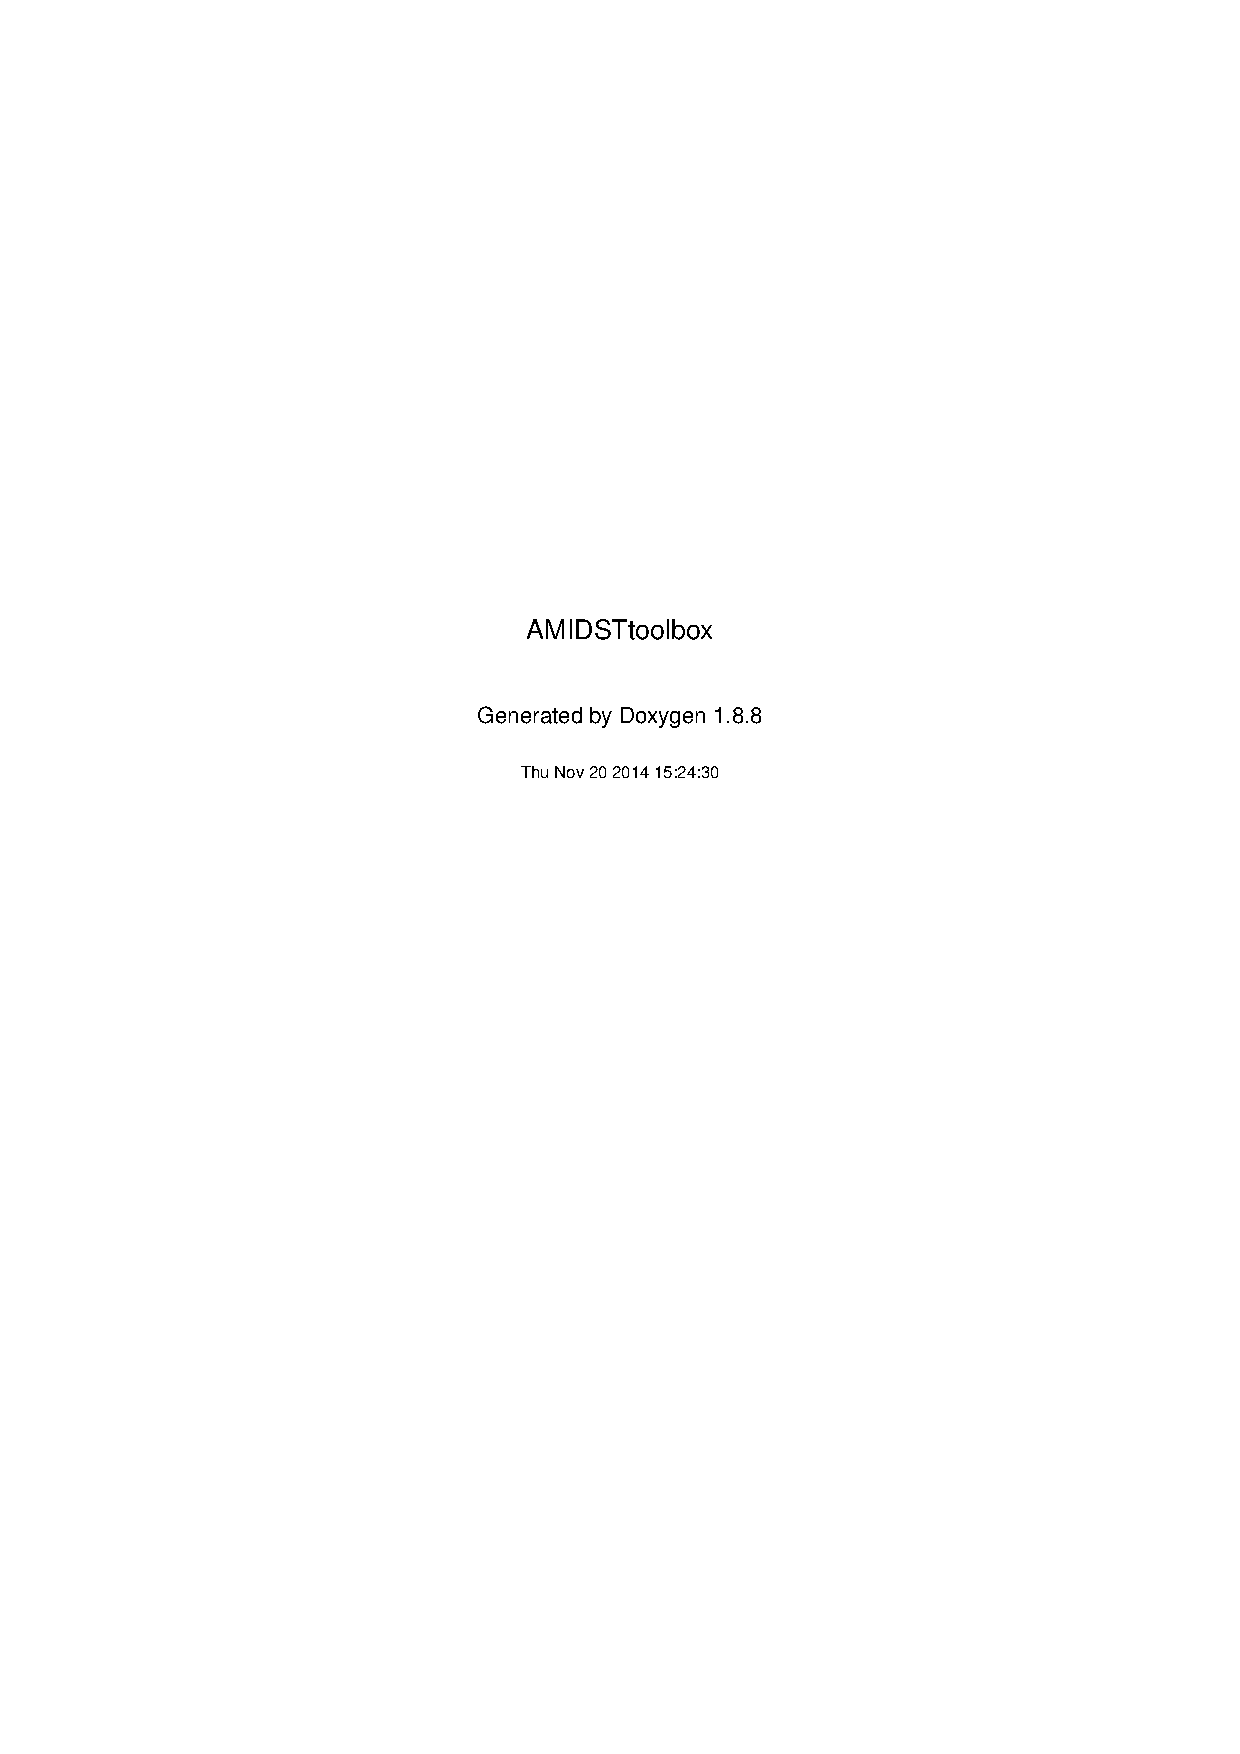
\includepdf[offset=0 1cm,scale=0.85,pages={-},pagecommand={\pagestyle{fancy}}]{doxygenPDF/refman.pdf}


\end{document}  